% !TeX spellcheck = hu_HU
\documentclass[12pt,a4paper]{article}
\usepackage[utf8]{inputenc}
\usepackage{cmap}
\usepackage[T1]{fontenc}
\usepackage[magyar]{babel}
\usepackage{amsmath}
\usepackage{amsfonts}
\usepackage{amssymb}
\usepackage{graphicx}

\usepackage{outlines}
\usepackage{hyperref}

\hyphenpenalty=10000

\begin{document}

\begin{center}
	\huge
	Telekommunikációs hálózatok\\
	\vspace{1mm}
	\LARGE
	Előadás és gyakorlat jegyzet\\
	\vspace{5mm}
	\large
	Készült Laki Sándor előadásai és gyakorlatai,\\
	valamint Gombos Gergő gyakorlatai alapján\\
	\vspace{5mm}
	Sárközi Gergő, 2022-23-1. félév\\
	Nincsen lektorálva!
\end{center}

\tableofcontents

\pagebreak

\section{Bevezetés}

\subsection{Alapfogalmak}

\begin{outline}
	\1 Végpont
		\2 (Hálózati) hoszt: eszköz, amely hálózattal össze van kötve
		\2 Szolgáltatásokat biztosíthat, információt oszt meg, stb.
	\1 Switch, router
	\1 Link (pl. WiFi, optikai szál, coax, RJ-45)
		\2 Átviteli csatorna, médium, közeg: amelyen kommunikáció folyik
	\1 Hálózati sávszélesség: elérhető/felhasznált kommunikációs erőforrás
		\2 Mértékegység: bit per second, SI váltószám: $10^3$ (IEC: $2^{10}$)
	\1 Internet: hálózatok hálózata
	\1 Hálózati folyam, flow: két fél közötti hálózati forgalom
		\2 Más definíció: valamilyen szempontból összetartozó forgalom
\end{outline}

\subsection{Topológiák}

\begin{outline}
	\1 Teljesen összekötött (Full-mesh)
	\1 Lánc/gyűrű
	\1 Busz: egy speciális link, ez ágazik le mindenhova
\end{outline}

\pagebreak

\subsection{Pár internet szolgáltatás technológia}

\subsubsection{Digital Subscriber Line (DSL)}

\begin{outline}
	\1 Telefon vonalon keresztül (nagy sávszélességű) internet háztartásba
	\1 3 csatorna
		\2 Letöltés: néhány 100 Mbps
		\2 Feltöltés: néhány 10 Mbps
		\2 Hang: 2 irány
	\1 Kapcsolatunk direkt egy nagyobb egységig (nincs megosztva)
\end{outline}

\subsubsection{Cable Access Technology (CATV)}

\begin{outline}
	\1 Koax TV kábellel (nagy sávszélességű) internet
	\1 2 csatorna
		\2 Letöltés: néhány 100 Mbps
		\2 Feltöltés: néhány 10 Mbps
	\1 Közeg meg van osztva háztartások között
\end{outline}

\subsubsection{Ethernet}

\begin{outline}
	\1 Leggyakoribb LAN (Local Area Network, helyi hálózat) technológia
	\1 Kábel: UTP+RJ45 vagy optikai+SFP
	\1 Sebesség: <1 Mbps-től >1 Gbps-ig (szimmetrikus, full-duplex)
	\1 Hálózati kártyába csatlakozik (NIC, Network Interface Controller)
\end{outline}

\subsubsection{Egyéb}

\begin{outline}
	\1 Telefon (pl. 4G)
	\1 Műholdas
	\1 Stb.
\end{outline}

\pagebreak

\subsection{Internet belseje}

\begin{outline}
	\1 Követelmények
		\2 Hibatolerancia: több útvonal források és célok között
		\2 Rugalmasság: linkek száma nem lehet túl nagy, meg kell osztani az erőforrásokat (költséghatékonyság és megvalósíthatóság érdekében)
		\2 Megfelelő csomópont kapacitás: linkek száma nem lehet túl kicsi
	\1 Kompromisszumos megoldás: switchelt/kapcsolt, csomagkapcsolt hálózatok
		\2 Előny: erőforrás megosztás van és csomópontok kapacitása igény szerint alakítható
		\2 Hátrány: a switch-nek okosnak kell lennie (csomagtovábbítás, forgalomirányítás, erőforrás kiosztás)
		\2 Linkek, switch-ek meg vannak osztva: egyszerre több flow is használja
	\1 Rendszerfüggetlenség, nincs központi felügyelet
	\1 Építőeleme a LAN
\end{outline}

\subsubsection{ISP (Internet Service Provider, Internet szolgáltató)}

\begin{outline}
	\1 Hierarchiában vannak
		\2 Tier-1 (interkontinentális), Tier-2 (nemzeti), Tier-3 (felhasználó)
		\2 Tier-1-nek nincsen szolgáltatója, ő csak szolgáltat
	\1 Peering link: ingyen van az adatátvitel rajta
		\2 Azonos tierek között
		\2 Nem használható akármire: a link egyik végén kell keletkeznie, a másikban terminálnia a forgalomnak
	\1 Transit link: fizetni kell a használt adatmennyiség után
		\2 pl. Tier-3 és Tier-2 között a Tier-2 fizet (szolgáltató-vásárló viszony)
	\1 Internet eXchange Point (IXP): sok ISP összekötése
		\2 Költséghatékony: egyszerre sok ISP találkozik, nem csak 1-1
\end{outline}

\pagebreak

\subsection{Erőforrás kezelés}

\subsubsection{Előre foglalás}

\begin{outline}
	\1 Folyam szintű multiplexálás
	\1 Előre lefoglal sávszélesség, amin aztán valamikor küld adatot
	\1 Több kiosztási módszer:
		\2 First-come first-served: első lefoglaló lefoglalhatja akár az egészet
		\2 Egyenlő elosztás: link sávszélessége egyenletesen el van osztva
	\1 Kihasználtság kiszámolása:
		\2 Legyen $P$ a csúcsráta (peak rate) és $A$ az átlagos ráta
		\2 Kihasználtsági szint: $A/P$ (pl. $P=100$ és $A=10$ esetén $10\%$)
		\2 Előre foglalás akkor jó választás, ha $P/A$ kicsi
			\3 Hang esetén általában ez az arány 3 vagy kevesebb
	\1 Megvalósítás: áramkörkapcsolt hálózat
		\2 Használja: vezetékes telefon hálózatok
	\1 Előnyök:
		\2 Egyszerű elveken alapuló gyors kapcsolás
		\2 Kiszámítható teljesítmény
	\1 Hátrány:
		\2 Hibatolerancia alacsony
		\2 Extra késleltetés: áramkör felépítése
		\2 Alacsony hatékonyság (sávszélesség pazarló)
\end{outline}

\subsubsection{Resource Reservation Protocol}

\begin{outline}
	\1 Áramkörkapcsolt hálózatok esetén egy erőforrás foglaló protokoll
	\1 1.: forrás foglalási kérést küld $X Mbps$ igényről a célállomásnak
	\1 2.: switchek kialakítják az "áramkört"
	\1 3.: forrás megkezdi az adatküldést
	\1 4.: forrás áramkör-lebontó üzenetet küld a célállomás felé (teardown)
\end{outline}

\pagebreak

\subsubsection{Igény szerinti}

\begin{outline}
	\1 Csomag szintű multiplexálás
	\1 Foglalás nélkül akkor küld adatot, amikor szükséges
	\1 Előre foglaláshoz képest általában nagyobb kihasználtság érhető el
		\2 Különbség függ: források számától, folyam börsztösségtől
		\2 Kommunikáció általában löketes (börsztös), $P/A$ jellemzően $100+$
	\1 Megvalósítás: csomagkapcsolt hálózat
		\2 Használja: internet
		\2 Minden csomag tartalmazza a cél címét/azonosítóját
	\1 Előnyök:
		\2 Hatékony erőforrás gazdálkodás
		\2 Egyszerű hálózatot készíteni, bővíteni
		\2 Hiba észlelése és kijavítása gyors, magas hibatolerancia
	\1 Hátrányok:
		\2 Kiszámíthatatlan teljesítmény
			\2 Ha túl sok csomag jön egyszerre, valami el lesz dobva
		\2 Bonyolult hardver kell: puffer-kezelés, torlódás-vezérlés
\end{outline}

\pagebreak

\subsection{Internet rétegmodelljei}

\begin{outline}
	\1 Internet célja: különböző eszközökön különböző folyamatok tudjanak kommunikálni egymással
	\2 Továbbá legyen hatékony, gyors, stb.
	\1 Protokoll és API kapcsolatban van
	\1 Sok a protokoll, stb.; megoldás: modularizáció, rétegződés
\end{outline}

\subsubsection{TCP/IP modell}

\begin{outline}
	\1 4 réteg
	\1 Link layer (kapcsolati réteg): 2 szomszédos pont közötti kommunikáció
		\2 Hardver közeli, itt még nem teljesen protokollokról beszélünk
		\2 Vastag réteg, sok minden történik itt (hibajavítás, stb.)
		\2 Pl. Ethernet
	\1 Internet layer (hálózati réteg): routing, 2 bármely pont közötti kommunikáció
		\2 Globális kommunikáció miatt nincs sokféle protokoll
		\2 Pl. IPv4, IPv6
	\1 Transport layer (szállítói réteg): processzek közötti kommunikáció
		\2 (De)multiplexálás (packet fragmentation and reassembly)
		\2 Alkalmazás követelmények biztosítása (pl. megbízhatóság)
		\2 Pl. TCP, UDP
	\1 Application layer (alkalmazási réteg): sztenderd alkalmazások ezt használják
		\2 Pl. socket api-n keresztül telnet szolgáltatás nyújtása
\end{outline}

\pagebreak

\subsubsection{ISO OSI referencia modell}

\begin{outline}
	\1 Open System Interconnection Reference Model, 7 réteg
	\1 Minden kommunikációs rendszert le tud írni (nem csak internetet)
	\1 Rétegek jellemzése
		\2 Szolgáltatás: mit csinál a réteg
		\2 Interfész: hogyan férünk hozzá a réteghez?
		\2 Protokoll: hogyan implementáljuk a réteget?
	\1 Fizikai réteg (physical layer):
		\2 Szolgáltatás: két fizikailag összekötött eszköz között adatátvitel
		\2 Interfész: specifikálja egy bit átvitelét
		\2 Protokoll: bit kódolási séma, feszültségi szintek, jelek időzítése
		\2 Példa: koaxiális kábel, optikai kábel
	\1 Adatkapcsolati réteg (data link layer):
		\2 Szolgáltatás:
			\3 Adat keretekre tördelése (pl. hibajavítás miatt)
			\3 Közeghozzáférés vezérlés (MAC) (pl. WiFi esetén)
			\3 Per-hop megbízhatóság és folyamvezérlés (pl. pause frame)
		\2 Interfész: keret küldése két közös médiumra kötött eszköz között
		\2 Protokoll: fizikai címzés, pl. MAC cím
		\2 Példa: Ethernet, WiFi
		\2 Sokszor összeforr a fizikai réteggel, általában nem függetlenek
	\1 Hálózati réteg (network layer): mint a TCP modellben
		\2 Szolgáltatás: csomagtovábbítás, útvonalválasztás, fragmentálás
			\3 Csomag ütemezés (priority queueing), puffer kezelés
		\2 Interfész: csomag küldése egy adott végpontnak
		\2 Protokoll: routing táblák karbantartása, globálisan egyedi címek
		\2 Példák: IPv4, IPv6
\pagebreak
	\1 Szállítói réteg (transport layer): mint a TCP modellben
		\2 Szolgáltatás: multiplexálás, megbízhatóság, sorrendhelyesség
			\3 Torlódásvezérlés: enélkül újraküldések miatt telítődne a puffer
		\2 Interfész: üzenet küldése cél processznek
		\2 Protokoll: port szám, folyamfelügyelet, megbízhatóság
		\2 Példa: UDP, TCP
	\1 Munkamenet réteg (session layer):
		\2 Ilyen nincsen az internetben, alkalmazásnak kell csinálni
		\2 Szolgáltatás: kapcsolat menedzsment, szinkronizációs pontok
		\2 Interfész: attól függ
		\2 Protokoll: token menedzsment, szinkronizációs checkpoint
	\1 Megjelenítési réteg (presentation layer):
		\2 Ilyen nincsen az internetben, alkalmazásnak kell csinálni
		\2 Szolgáltatás: adatkonverzió különböző reprezentációk között
			\2 pl. ascii-unicode vagy endianness (little-big)
		\2 Interfész: attól függ
		\2 Protokoll: adatformátum és transzformációs szabályok
	\1 Alkalmazási réteg (application layer): bármi
\end{outline}

\subsubsection{Hibrid TCP/IP modell}

\begin{outline}
	\1 5 réteg: OSI mínusz session, presentation (a 2 nem implementált)
	\1 Mi ezt használjuk, Tanenbaum és mások találták ki
	\1 L1 physical: fizikai bit továbbítás (twisted pair, fiber)
	\1 L2 link: lokális best-effort továbbítás (Ethernet, Wifi)
	\1 L3 network: globális best-effort továbbítás (IP)
	\1 L4 transport: végpontok (processzek) közötti továbbítás (TCP, UDP)
	\1 L5 application: magas szintű hálózat hozzáférés (HTTP, FTP)
\end{outline}

\pagebreak

\subsection{Rétegek alkalmazása}

\begin{outline}
	\1 IP réteg a legszűkebb: ezen a ponton egységes protokoll kell globalitáshoz
	\1 Rétegek adategysége (protocol data unit, PDU):
		\2 L1 physical: bit
		\2 L2 data link: frame (keret)
		\2 L3 network: packet (csomag)
		\2 L4 transport: segment (szegmens)
		\2 L5 application: message (üzenet)
	\1 Első 2-3 réteget minden eszköz implementálja
		\2 Szállítói, alkalmazási réteg általában a végpontokban van implementálva
		\2 Kivétel: pl. olyan tűzfal, ami ezeket figyelembe veszi
		\2 Switch: első 2 réteget tudja; router: első 3 réteg
	\1 L2 - L4 akár szoftveres, akár hardveres is lehet
		\2 L4 transport hardverben: smartNIC (TCP rásegítés)
		\2 L3 network: NIC vagy szoftveres routing tábla
		\2 L2 link: általában NIC (vagy switch), de pl. virtuális hálózat
		\2 Hardver gyorsabb, szoftver flexibilisebb, de ez a határ kezd elmosódni
			\3 SDN, P4 hardver oldalról; DPDK szoftver oldalról
	\1 Rétegek egymást enkapszulálják: a réteg/protokoll fejlécét odarakjuk a többi mellé, legvégén pedig a payload van
		\2 Kivétel: Ethernet a csomag végére, payload után is rak
		\2 Switchek, routerek egyes fejléceket módosítanak, de a többit békén hagyják és csak tovább küldik
\end{outline}

\pagebreak

\subsection{Hálózatok karakterizációja}

\begin{outline}
	\1 Három szempont:
		\2 Késleltetés, delay
		\2 Csomagvesztés, loss
		\2 Fogadási adatráta, throughput
\end{outline}

\subsection{Késleltetés, delay}

\begin{outline}
	\1 Total delay = transmission + propagation + processing + queueing
		\2 transmission, propagation: linktől függ
			\3 Melyik fontosabb? Helyzettül függ
			\3 Kicsi csomag: propogation miatt lesz lassú
			\3 Nagy csomag: transmission miatt lesz lassú
		\2 processing, queueing: switchtől, switchen adatforgalomtól függ
	\1 Propagation delay = link length / signal propagation speed
		\2 Rézkábel: 2/3 fénysebesség
		\2 Optikai kábel: 2/3 fénysebesség (fény pattog; út nem egyenes)
		\2 Fénysebesség konstans, ezért csökkentésre: Content Delivery Network
			\3 Közelebből kelljen az információt elküldeni a célba
	\1 Transmission delay: 1 Gbps link esetén 1 bit kiírása $10^{-9}s$
	\1 Queueing delay: pufferben töltött idő
		\2 Nehéz megbecsülni, csomagonként változik
		\2 Mérőszámok: átlag, variancia, esély X feletti értékre
		\2 Függ: érkezési ráta, küldési ráta, traffik börsztösség
		\2 Traffik intenzitás = csomag bitméret * érkezési pps / küldési bps
			\3 Ha ez nagyobb mint 1, akkor idővel biztosan tele lesz a puffer
		\2 Delay felső korlát: puffer méret * csomag bitméret * küldési bps
\end{outline}

\pagebreak

\subsection{Loss (csomageldobás, csomageldobódás)}

\begin{outline}
	\1 Ha teli a puffer és jön egy újabb packet, akkor valamit el kell dobni
		\2 El lehet dobni az új csomagot
		\2 El lehet dobni a puffer legrégebbi csomagját
		\2 Létezik priority queueing (QoS, quality of service)
	\1 Miért lehet teli a puffer?
		\2 Pillanatnyilag nagyon nagy börszt van
		\2 A traffik intenzitás értéke 1-nél több (több adat jön, mint megy)
\end{outline}

\subsection{Throughput, (lehetséges maximum) sávszélesség}

\begin{outline}
	\1 Throughput (bps) = adat méret (bit) / átviteli idő (s)
		\2 Több linkból álló lánc esetén a legkisebb értékű link számít
		\2 Optimálisan több TCP stream: sávszélesség egyenletesen eloszlik
		\2 TCP: megtalálja a bottleneck-et (nagy fluktuációval)
\end{outline}

\pagebreak

\section{Fizikai réteg (physical layer)}

\subsection{Áttekintés}

\begin{outline}
	\1 Szolgáltatás: két fizikailag összekötött eszköz között adatátvitel
	\1 Interfész: specifikálja egy bit átvitelét
	\1 Protokoll: bit kódolási séma, feszültségi szintek, jelek időzítése
	\1 Példa: koaxiális kábel, optikai kábel
\end{outline}

\subsection{Elméleti alapok}

\begin{outline}
	\1 Küldeni könnyű, de a fogadó félnek torz jelet kell tudni értelmezni
	\1 Jel elnyelődés, signal attenuation
		\2 Fogadó túl kevés energiájú, túl tompa jelet kap
		\2 Frekvenciafüggő: más frekvenciák máshogy nyelődnek el
			\3 A jelünk több frekvenciából áll, ez ezért probléma
		\2 Távolság növelésével nő az elnyelődés
		\2 Megoldás: vannak frekvencia sávok közelítőleg egyenletes elnyelődéssel
			\3 Ezek a sávok a közegtől függenek
		\2 Számolása: $\alpha \; [dB] = 10 dB \times \log_{10} \frac{\text{küldési energia}}{\text{vételi energia}}$
	\1 Fáziseltolódás: más frekvenciájú a hullámok terjedési sebessége eltér
	\1 Zaj: hő, más rendszerek (mikrohullámú sütő)
	\1 Adatátvitel valamilyen fizikai jellemző (pl. feszültség, áramerősség) változtatásával lehetséges
		\2 Különböző frekvenciájú szinuszhullámok végtelen sörösszegével mindenféle periodikus jel felírható
\end{outline}

\pagebreak

\subsection{Szimbólumok, bitek}

\begin{outline}
	\1 Bitek helyett szimbólumokat küldünk
	\1 Azonos küldési rátával magasabb sávszélesség érhető el
		\2 Mert 2 helyett több jelszint (pl. 4) használható
		\2 Olyan fogadó kell, ami meg tudja különböztetni a több jelszintet
	\1 Két mérőszám: adat ráta (bps) és szimbólum ráta (Baud, symbols/sec)
\end{outline}

\subsection{Átviteli közegek}

\subsubsection{Vezetékes}

\begin{outline}
	\1 Egy kamion tele HDD-vel (azaz mágneses adathordozók)
		\2 Magas sávszélesség, nagy késleltetés
	\1 Sodort érpár (twisted pair), pl. UTP
		\2 Analóg és digitális jel átvitelére is alkalmas
	\1 Koaxiális kábel: sodort érpárhoz képest nagyobb sebesség és távolság
		\2 Sodrás helyett egyenes kábel + fonott külső "Faraday kalitka"
		\2 Kétharmad fénysebesség van a rézszál közegben
	\1 Optikai szál (kétharmad fénysebességre képes pattogás miatt)
\end{outline}

\pagebreak

\subsubsection{Vezeték nélküli}

\begin{outline}
	\1 Elméleti alapok, $\lambda f = c$
		\2 Frekvencia ($f$, Hz): EM hullám másodpercenkénti rezgésszáma
		\2 Hullámhossz ($\lambda$, m): két egymást követő hullámcsúcs távolsága
		\2 Fénysebesség ($c=3*10^8 \frac{m}{s}$): EM terjedési sebessége vákuumban
	\1 Rádiófrekvenciás átvitel
		\2 Egyszerű, használható bel- és kültéren, frekvenciafüggő terjedés
		\2 Alacsony frekvencia: nagy távolság, kis sávszélesség
		\2 Alacsony frekvenciás jel visszapattan az ionoszféráról, így a föld görbületét "meg lehet oldani"
	\1 Mikrohullámú átvitel
		\2 Egyenes vonal mentén terjed, elnyelődés egy probléma, olcsó
	\1 Infravörös és milliméteres hullámú átvitel
		\2 Kis távolságra képes, szilárd testeken nem hatol át
	\1 Látható fényhullámú átvitel (lézerforrás és fényérzékelő)
		\2 Olcsó, nagy sávszélesség, nem engedélyköteles
		\2 Időjárás erősen befolyásolja
	\1 Kommunikációs műholdas átvitel: annyira nem fontos
		\2 Magas pálya: nagy területet képes kiszolgálni, de nagyobb a késleltetés
		\2 Starlink: alacsony pálya, minimális késleltetés, rengeteg műhold
\end{outline}

\pagebreak

\subsection{Adatátvitel}

\subsubsection{Kiinduló feltételek}

\begin{outline}
	\1 Két jelszint van: magas (1) és alacsony (0)
	\1 Szinkron átvitel: egy óra vezérli a mintavételezést
	\1 Jel amplitúdója és időbeli kiterjedése számít
\end{outline}

\subsubsection{Non-Return to Zero (NRZ) kódolás}

\begin{outline}
	\1 1-es bit esetén magas jel, 0-as bit esetén alacsony jel
	\1 Előny: hatékony
	\1 Probléma: hosszú azonos jelszint esetén elveszik az adó és a vevő közötti szinkronizáció
	(hogy mikor kell mintavételezni)
		\2 Ha egy kicsit el tud csúszni az óra, akkor előbb utóbb el tud csúszni annyira, hogy egy teljes bit kimaradjon
	\1 Probléma: "nincs jel" és "sok nulla jön" nem nagyon tér el egymástól
\end{outline}

\subsubsection{Szinkronizáció lehetőségek}

\begin{outline}
	\1 Explicit órajel küldése egy párhuzamos átviteli csatornán
	\1 Kritikus időpontokban szinkronizáció (pl. szimbólum/blokk kezdetén)
	\1 Szimbólum kódok: szignál tartalmazza szinkronizáláshoz szükséges infót
		\2 Önütemező jel, azaz külön órajel nélkül dekódolható
\end{outline}

\subsubsection{Manchester kódolás (10 Mbps Ethernet)}

\begin{outline}
	\1 1-es bit: átmenet magasról alacsonyra
	\1 0-ás bit: átmenet alacsonyról magasra
	\1 Probléma: 1 bithez 2 óraidő ciklus szükséges (akár 2 átmenet kell)
\end{outline}

\pagebreak

\subsubsection{Non-Return to Zero Inverted (NRZI) kódolás}

\begin{outline}
	\1 1-es bit esetén átmenet, 0-as bit esetén nincs változás
	\1 Előny: hatékony
	\1 Probléma: csupa 0 bit sorozat esetén ugyanúgy elveszhet a szinkronizáció
\end{outline}

\subsubsection{4-bit/5-bit kódolás NRZI előtt (100 Mbps Ethernet)}

\begin{outline}
	\1 Minden 4 hosszú bitsorozat 5 hosszúra kódolása
		\2 Nem lehet 1-nél több 0 az elején
		\2 Nem lehet 2-nél több 0 a végén
		\2 kódolás megoldható egy $16=2^4$ elemű táblázattal
	\1 Hátrány: 80\%-os hatékonyság NRZ-hez képest
	\1 Előny: nincs többé szinkronizáció elvesztés
\end{outline}

\subsubsection{8-bit/10-bit kódolás NRZI előtt (Gigabit Ethernet)}

\begin{outline}
	\1 Ugyan az, mint a 4-bit/5-bit, csak más mennyiségű bitet map-el
\end{outline}

\subsection{Jelátvitel}

\begin{outline}
	\1 Digitális esetben véges halmazzal dolgozunk, így van lehetőségünk hibajavításra
\end{outline}

\begin{figure}[h!]
	\centering
	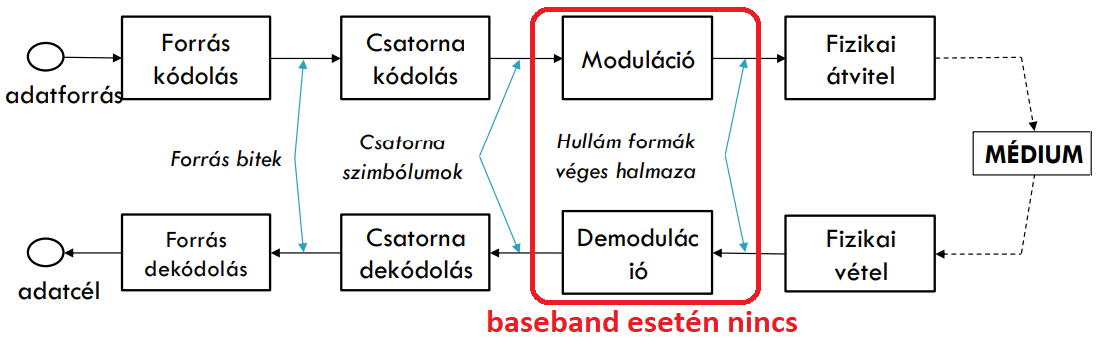
\includegraphics[width=0.8\linewidth]{baseband-vs-broadband}
\end{figure}

\subsubsection{Alapsáv, baseband (korlátos technológia)}

\begin{outline}
	\1 Digitális jel árammá vagy feszültséggé alakul
	\1 Jel minden frekvencián a sávon belül átvitelre kerül
\end{outline}

\pagebreak

\subsubsection{Szélessáv, broadband}

\begin{outline}
	\1 Széles frekvenciatartományban történik az átvitel
	\1 Egy vivőhullám mindig ott van a közegen, ezt változtatjuk meg
	\1 Modularizáció, vivőhullámba a digitális jel kódolásának lehetőségei:
		\2 Amplitúdó Moduláció (AM): adatok vivőhullámra ültetése
		\2 Frekvencia (FM) vagy fázis moduláció: vivőhullám változtatása
		\2 Különböző vivőhullámok egyidejűleg felhasználása
\end{outline}

\begin{figure}[h!]
	\centering
	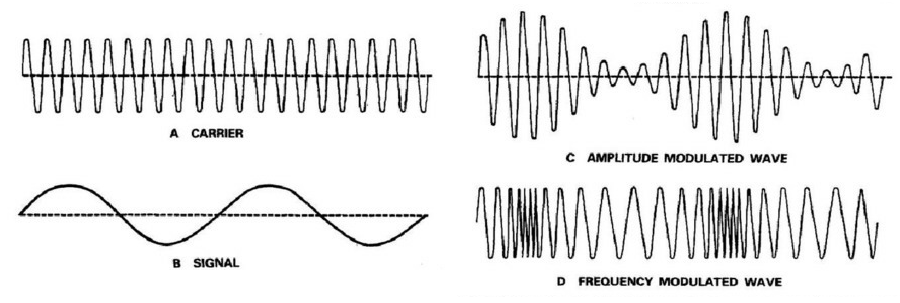
\includegraphics[width=1\linewidth]{carrier-signal-am-fm}
\end{figure}

\subsubsection{Amplitúdó Moduláció (AM)}

\begin{outline}
	\1 Digitális szignál: amplitúdó-eltolás keying (szimbólumonként más amplitúdó)
	\1 $f_A(t) = s(t)*\sin(2 \pi f t + \varphi)$
\end{outline}

\subsubsection{Frekvencia Moduláció (FM)}

\begin{outline}
	\1 Digitális: frekvencia-eltolás keying (szimbólumonként különböző frekvencia)
	\1 $f_F(t) = \alpha*\sin(2 \pi s(t) t + \varphi)$
\end{outline}

\pagebreak

\subsubsection{Fázis moduláció}

\begin{outline}
	\1 Analóg esetben nem működik túl jól
	\1 $f_P(t) = a * \sin(2 \pi f t + s(t))$
	\1 Digitális szignál: fázis-eltolás keying (PSK)
	\1 Quadrature Phase Shift Keying (QPSK)
		\2 Diszkrét halmaz kódolja a szimbólumokat
		\2 4 szimbólum $\implies$ kétszeres adatráta a szimbólumrátához képest
\end{outline}

\begin{figure}[h!]
	\centering
	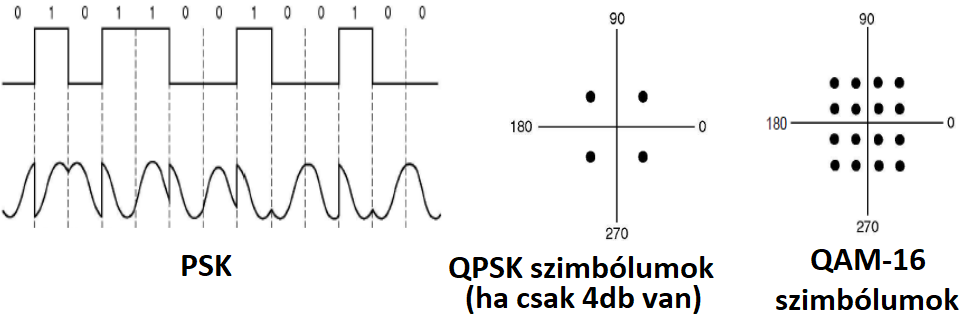
\includegraphics[width=0.75\linewidth]{phase-modulation-and-qam}
\end{figure}

\subsubsection{Quadrature Amplitude Modulation (QAM)}

\begin{outline}
	\1 Kombinálja az amplitúdó és a fázis modulációt
	\1 Diszkrét halmaz kódolja a szimbólumokat
		\2 16 szimbólum $\implies$ négyszeres adatráta szimbólumrátához képest
	\1 Máshogy felfogva: két merőleges (90-fokkal eltolt), azonos frekvenciájú hullámot amplitúdó modulálunk, ezzel koordinátákat írva le
\end{outline}

\pagebreak

\subsection{Multiplexálás}

\begin{outline}
	\1 Statikus csatorna hozzáférés módszereket nézünk (statikus allokáció)
	\1 Egy fizikai közegen több jel párhuzamosan utazik
		\2 Fizikai csatornát logikai alcsatornákra bontjuk
	\1 Küldő oldalon kell speciális eszköz (multiplexer), ami a jelet a megfelelő alcsatornára helyezi
\end{outline}

\subsubsection{Térbeli multiplexálás (space-division multiplexing)}

\begin{outline}
	\1 Minden csatornához külön fizika eszköz
		\2 Vezetékes átvitel: külön pont-pont vezeték
		\2 Vezeték nélküli átvitel: külön antenna
	\1 Celluláris hálózatokra jellemző
\end{outline}

\subsubsection{Frekvencia multiplexálás (frequency-division multiplexing)}

\begin{outline}
	\1 Szignálonként más frekvencia, közöttük "guardband"
	\1 Analóg esetben szokás alkalmazni
	\1 Többféle megvalósítás létezik:
		\2 Direct Sequence Spread Spectrum: szignálon XOR véletlen bitsorozattal
		\2 Frequency Hopping Spread Spectrum: pszeudo véletlen alapú választás sok frekvencia közül (mindkét fél ismeri a pseudo véletlen seed-jét)
\end{outline}

\subsubsection{Hullámhossz multiplexálás (wavelength-division multiplexing)}

\begin{outline}
	\1 Gyakorlatilag frekvencia multiplexálás, csak optikai szálon
\end{outline}

\subsubsection{Időbeli multiplexálás (time-division multiplexing, TDM)}

\begin{outline}
	\1 Minden állomás kap egy diszkrét időszeletet (slot)
	\1 Koordináció vagy merev felosztás szükséges
\end{outline}

\pagebreak

\subsubsection{Code Division Multiple Access (CDMA)}

\begin{outline}
	\1 3G-s mobilhálózatok alapja, mobil kommunikációban elterjedt
	\1 1 bitnyi információ helyett $m$ bitnyi információt küldünk
	\1 Minden állomás sugározhat akár folyamatosan, párhuzamosan
	\1 Minden állomáshoz tartozik egy töredéksorozat (chip sequence), ami egy $m$ bites kód
		\2 Ezek a kódok ortogonális bázist alkotnak
	\1 Egy állomás mit küldjön, ha egy adott bitet akar továbbítani?
		\2 1-es bit küldése esetén az állomás elküldi a kódját
		\2 0-ás bit küldése esetén a kódjának az egyes komplemensét
	\1 Ortogonális bázis miatt az interferált jelből csak projekciót kell végezni
\end{outline}

\pagebreak

\section{Adatkapcsolati réteg (data link layer)}

\subsection{Áttekintés}

\begin{outline}
	\1 Szolgáltatás:
		\2 Adat keretekre tördelése (pl. hibajavítás miatt)
		\2 Közeghozzáférés vezérlés (MAC) (pl. WiFi esetén)
		\2 Per-hop megbízhatóság és folyamvezérlés (pl. pause frame)
	\1 Interfész: keret küldése két közös médiumra kötött eszköz között
	\1 Protokoll: fizikai címzés, pl. MAC cím
	\1 Példa: Ethernet, WiFi
	\1 Sokszor összeforr a fizikai réteggel, általában nem függetlenek
\end{outline}

\subsection{Keret képzés, keretezés, framing}

\begin{outline}
	\1 Csomag-kapcsolt hálózat: csomagok routing információt is tartalmaznak
		\2 Azaz van fejléc, azaz ismerni kell az adathatárokat
	\1 Nincs hibamentesség $\implies$ kell hiba felismerés és/vagy javítás
		\2 Nagy keret méret $\implies$ hiba valószínűbb
	\1 Megbízható időzítésre nincs nagyon lehetőség
\end{outline}

\subsubsection{Bájt alapú: karakterszámlálás}

\begin{outline}
	\1 Fejléc tárolja a keretben lévő karakterek számát
	\1 Probléma: ha a karakterszámban történik hiba, akkor az egész szétcsúszik
\end{outline}

\subsubsection{Bájt alapú: bájt beszúrás (byte stuffing)}

\begin{outline}
	\1 FLAG speciális bájt (jelölő bájt) jelzi a keret elejét és végét
		\2 ESC speciális bájt-tal escape-elni kell az adaton belül
		\2 ESC-et is ESC-elni kell
	\1 Legrosszabb esetben kb. megkétszereződik az hossz
	\1 Használat: pont-pont alapú protokollok, pl. modem, DSL, cellular
\end{outline}

\pagebreak

\subsubsection{Bit alapú: bit beszúrás (bit stuffing)}

\begin{outline}
	\1 Minden keret speciális bitmintával kezdődik és végződik: 0\textbf{11}11\textbf{11}0
	\1 Minden 5db 1-es bit küldése után egy 0-ás bit lesz beszúrva
	\1 Fogadásnál 11111 bitsorozat kezelése:
		\2 Következő bit 0: ez a 0 figyelmen kívül hagyása (beszúrás eredménye)
		\2 Következő bitek 1 majd 0: keret vége
		\2 Következő bitek 1 majd 1: keret eldobása, mert ez nem történhetne
			\3 Ez attól még nem egy hibadetektáló módszernek számít! 
	\1 Legrosszabb esetben 20\%-os hossz növekedés
	\1 Egyes hardverekben nehezebb megcsinálni a bit műveleteket
\end{outline}

\subsubsection{Óra alapú keretezés: SONET (Synchronous Optical NETwork)}

\begin{outline}
	\1 Optikai kábelen gyors átvitelt valósít még
	\1 STS-n a nevük, most ezt nézzük: STS-1, 51.84 Mbps
	\1 Minden keret pontosan 125$\mu s$ hosszan tart, $9*90=810$ bájtosak
		\2 Van keret kezdő mintázat
	\1 Fizika részhez tartozik:
		\2 NRZ kódolás van használva
		\2 Speciális 127 bites mintával van XOR-olva az adat, hogy kevés hosszú 0 és 1 sorozat legyen
\end{outline}

\pagebreak

\subsection{Hibafelügyelet}

\begin{outline}
	\1 Zajforrások: kábelek között interferencia, rádiós áthallás, mikrosütő
	\1 Hibák általában börsztösek (mert az interferencia általában ideig tart)
		\2 Neve: csoportos hiba (burst error)
		\2 $m$ paraméter: védelmi övezet (guard band)
			\3 Egy csoporton belül két hibás bit között max $m-1$ helyes bit
			\3 Ellenkező esetben nem egy, hanem két csoportról beszélünk
		\2 Másik lehetőség: egyszerű bithiba (1 bit)
	\1 Redundancia nélkül nincs lehetőség hibajavításra, hibadetektálásra
\end{outline}

\subsubsection{Hiba vezérlés}

\begin{outline}
	\1 Stratégiák
		\2 Hiba javítás (hiba javító kódok, forward error correction)
			\3 Akkor is működik, ha szinte minden keret hibás
			\3 Nagyobb az overhead
			\3 Hibajavítás mértéke változtatható pl. távolság függvényében
		\2 Hiba detektálás és újraküldés
			\3 ARQ: Automatic Repeat Request
			\3 Megbízható csatornán hatékonyabb
			\3 Gyakorlatban elterjedt
			\3 Semmire nem jó, ha szinte minden keret hibás
	\1 Hiba javítás detektálás nélkül: pl. hangátvitel esetén lehetőség
\end{outline}

\subsubsection{Naiv hibadetektálás}

\begin{outline}
	\1 Minden keretben az adat kétszer legyen benne
		\2 Nem hatékony a méret növekedéshez képest
		\2 Kétszer akkora keret $\implies$ hibák számának várható értéke duplázódik
	\1 Paritás bit: +1 bit az adathoz, hogy az 1-es bitek száma páros legyen
		\2 1 bites hibák detektálhatok, de 2 bites hiba már nem
		\2 Börsztös hibák ellen nem megbízható
\end{outline}

\pagebreak

\subsubsection{Redundancia}

\begin{outline}
	\1 Redundancia nélkül lehetetlen a hibafelismerés
		\2 Magasabb absztrakciós szinten igen, pl. HTTP szintaxis ellenőrzés
	\1 Keret felépítése ($n$ bit): $m$ adat bit + $r$ redundáns/ellenőrző bit
		\2 Elnevezés: $n$ hosszú kódszó
	\1 Hamming távolság: (ez egy metrika)
		\2 Kódszavak esetén: $d(x,y) = $ bitek száma, ahol $x$ és $y$ különbözik
		\2 Kódszavak halmaza: $d(S)= \min_{x,y \in S \wedge x \ne y} d(x,y)$
	\1 $d(S)=d \implies$ $d-1$ hiba felismerhető, $\lfloor \frac{d-1}{2} \rfloor$ hiba javítható
		\2 Azaz $d$ bit hiba felismeréséhez $d+1$ Hamming távolság kell
		\2 Azaz $d$ bit hiba javításához $2d+1$ Hamming távolság kell
	\1 Hamming korlát (bináris kódkönyvre):
		\2 Legyen $C \subseteq \{0,1\}^n$ és $d(C)=k \in \mathbb{N}_+$
		\2 Ekkor $|C| * \sum_{i=0}^{\lfloor (k-1)/2 \rfloor}\binom{n}{i} \le 2^n$
		\2 Jelentése: |kijavítható kódszavak| $\le$ |lehetséges kódszavak|
		\2 Ha egyenlőség áll fenn: Perfekt-kód
		\2 Bizonyítások: polinom jegyzet,\\
		https://github.com/Trigary/uni-notes/tree/master/dimat2
	\1 Jó kódnak a rátája és a távolsága is nagy
		\2 Ráta: $R_S=\frac{\log_2 |S|}{n}$ (hatékonyságot karakterizálja)
		\2 Távolság: $\delta = \frac{d(S)}{n}$ (hibakezelési lehetőségeket karakterizálja)
\end{outline}

\pagebreak

\subsubsection{Hamming-kód}

\begin{outline}
	\1 $2$ hatványai pozíciókban ellenőrző bitek (1,2,4,8,...)
		\2 A többi pozícióban vannak az adatbitek
		\2 Az első bit az 1-es pozícióban van
		\2 Ebből következik, hogy paritás bit csak a saját csoportjába tartozik
	\1 Mindegyik ellenőrző bit paritás bit: párosra/páratlanra állítja a csoportot
		\2 Ez alapján even parity-ről vagy odd parity-ről beszélünk
		\2 Általában even parity-t használunk (legyen páros a darabszám)
	\1 $k$-adik bitet mi ellenőrzi: $k$ 2 hatványok összegeként felírva sorszámúak
		\2 pl. $k=13 \implies k=1+4+8 \implies$ 1-es, 4-es és 8-as paritás bit
		\2 Ez a $k$ ez a paritás biteket is tartalmazó kódszóban a sorszám
	\1 Példa (even parity-vel): 1000101 $\to$ \textbf{1}\textbf{0}1\textbf{0}000\textbf{0}101
	\1 Fogadás, dekódolás (1 bit hiba javítható)
		\2 Számláló 0-ról indul, $k$-nál nem jó a paritás bit $\implies$ k-t ad hozzá
		\2 Ha a számláló 0, akkor nincs detektálva hiba
		\2 Ha a számláló $j$, akkor a $j$-edik bitet meg kell fordítani
\end{outline}

\pagebreak

\subsubsection{CRC kód (Cyclic Redundancy Check)}

\begin{outline}
	\1 Egy polinom kód (bitsorozat felfogható $\mathbb{Z}_2$ feletti polinomként)
	\1 (CRC) checksum magyarul: (CRC) ellenőrző összeg
		\2 Ez kerül az átküldendő adat után az üzenet végére
\end{outline}

\begin{figure}[h!]
	\centering
	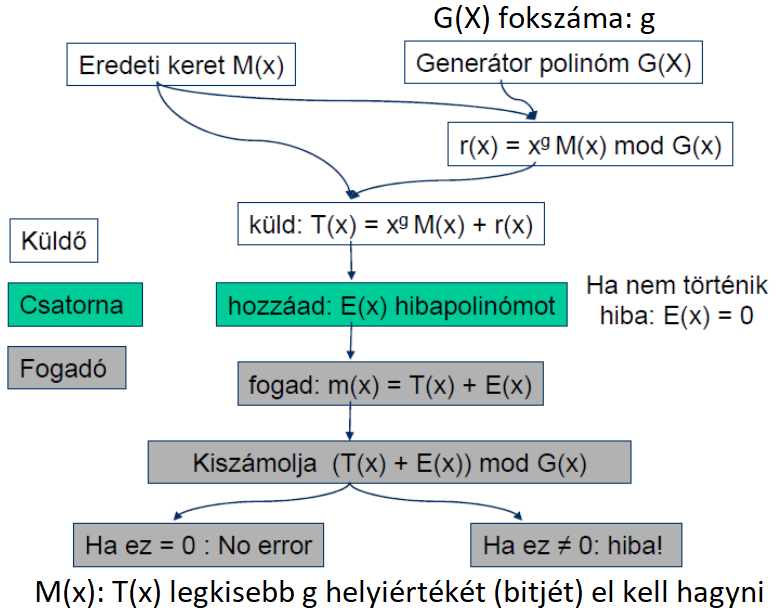
\includegraphics[width=0.6\linewidth]{crc}
\end{figure}

\begin{outline}
	\1 $G(x)$ többszöröseinek megfelelő hibákat nem ismerjük fel
	\1 $\deg G \ge 2 \implies$ minden egybites hibát észrevesz ($E(x)=x^i$)
	\1 Minden 2 bites hibát észrevesz, ha
		\2 $G(x)$ nem osztható $x$-szel
		\2 $G(x)$ nem osztható $x^k+1$-gyel, ahol $k < \deg M(x)$
	\1 $G(x)$ az $x+1$ többszöröse $\implies$ minden páratlan számú bithiba felismerhető
	\1 $G(x)$ legmagasabb, legalacsonyabb fokú tagjai együtthatója legyen 1
		\2 Ekkor lesz a CRC működőképes, jó, hatékony
	\1 Egy jó $G(x)$ minden max $\deg G$ hosszú csoportos hibát felismer
		\2 Emlékeztető: $G(x)$ többszöröseinek megfelelő hibák nem felismerhetők
\end{outline}

\pagebreak

\subsection{Forgalomszabályozás (flow control)}

\begin{outline}
	\1 Cél: gyors adó, lassú vevő probléma ne lépjen fel (elárasztás)
	\1 Visszacsatolás alapú forgalomszabályozás (feedback-based flow control)
		\2 Fogadó engedélyezi az adónak, hogy küldhet
		\2 Alternatíva, adatkapcsolati rétegben nem szokás:
			\3 Sebesség alapú forgalomszabályozás, rate-based flow control
			\3 Protokollba integrált sebességkorlát
	\1 Továbbiakban: fejrészben vezérlési infók, lábrészben ellenőrző összeg
	\1 Kommunikáció fajták:
		\2 Szimplex: kommunikáció egy irányba lehetséges
		\2 Fél-duplex: egyszerre csak egy irány, de egyébként kettő
		\2 Duplex: mindkét irányba szimultán kommunikáció lehetséges
\end{outline}

\subsubsection{Korlátozás nélküli szimplex protokoll}

\begin{outline}
	\1 Küldő csak küld végtelenségig, vevő csak fogad, puffer méret végtelen
	\1 Nincs meghibásodás/csomagvesztés, nincs sorszámozás, nincs nyugta
\end{outline}

\subsubsection{Szimplex megáll-és-vár protokoll (stop-and-wait)}

\begin{outline}
	\1 Előzőhöz képest különbség: adó és vevő eltérő sebességgel működik
	\1 Küldő küld egy keretet és vár, amíg a fogadó nyugtát nem küld
		\2 Tehát fél-duplex csatorna kell
	\1 Alacsony csatorna kihasználtság (pl. magas propagation delay esetén)
\end{outline}

\subsubsection{Szimplex protokoll zajos csatornákhoz (igazi megáll-és-vár)}

\begin{outline}
	\1 Előzőhöz képest különbség: van csomagvesztés és hibásodás
	\1 Egy keretet csak akkor adunk a hálózati rétegnek tovább, ha nem hibás
		\2 Hiba esetén a keret el van dobva és nincsen nyugta küldve
		\2 Tehát küldő oldalon kell "timeout", azután ismételt küldés
	\1 Nyugta (ACK) vesztés esetén hálózati rétegbe duplikált keret kerül
\end{outline}

\subsubsection{Alternáló-bit protokoll (ABP)}

\begin{outline}
	\1 Duplikátum probléma megoldása: 1 bites sorszám bevezetése
	\1 Küldő küld egy keretet és vár egy nyugtára (vagy timeout-ol)
		\2 Kezdő sorszám 0; nyugta megérkezése esetén megnöveli (mod 2)
		\2 Timeout esetén újraküldés (azonos sorszámmal)
	\1 Vevő vár egy hiba nélküli keretet (hibás keretet eldobja)
		\2 Keretet továbbadja hálózati rétegnek, küld nyugtát, léptet sorszámot
	\1 Alacsony csatorna kihasználtság: nincs megoldva
		\2 Csatorna kihasználtság: $\eta = \frac{T_{packet}}{T_{packet} + d + T_{ack} + d}$
			\3 $T_{xyz}$: keret kiküldéséhez szükséges idő; $d$: propagation delay
		\2 Magas propagation delay esetén $\eta$ alacsony (nem hatékony)
		\2 Protokoll megtartásával hatékonyság növelés: keretméret növelése
\end{outline}

\subsubsection{Csúszó-ablak protokollok általános jellemzői}

\begin{outline}
	\1 Pipeline technika: nem várunk minden egyes keret után nyugtára
	\1 Ablak (és puffer) méret: $n$ (max párhuzamos nyugtázatlan keretek)
	\1 Sorszám: sorozatban hányadik a keret
		\2 Adási/vételi ablak: küldhető/fogadható sorszámok halmaza
		\2 Adási ablak küldéskor szűkül, nyugta érkezésével nő
	\1 Kumulatív nyugtázás: minden kisebb sorszámú keretet nyugtáz
		\2 Nyugta tartalmazza a következőnek várt keret sorszámát
		\2 Hibás keretet eldobjuk és nem küldünk nyugtát
		\2 Nem megengedett sorszámú keretet eldobjuk, de nyugtázzuk:\\
		mert ilyen akkor történhet, ha egy nyugta veszett el
	\1 Küldő oldalon van timeout (és újraküldés)
	\1 Duplex csatorna kell (gyakorlatban mindenképpen, elméletben határeset)
		\2 Piggybacking, kétirányú kommunikáció: adatkeret fejlécben a nyugta
		\2 Piggybacking magyarul: hátizsák
	\1 Mi van, ha hosszú küldési sorozat közepén van a hiba?
\end{outline}

\pagebreak

\subsubsection{Csúszó ablak stratégia: visszalépés N-nel (go-back-n)}

\begin{outline}
	\1 Összes hibás keret utáni keret eldobása, nyugtázás nélkül
	\1 Küldő a timeout után újraküld minden keretet a hibástól kezdve
	\1 Nagy a hibaarány $\implies$ nem hatékony
\end{outline}

\subsubsection{Csúszó ablak stratégia: szelektív ismétlés (selective repeat)}

\begin{outline}
	\1 Hibás keretet eldobja, de utána minden hiba nélküli keretet pufferel
	\1 Küldő a timeout után újraküldi a hibás keretet
	\1 Nyugta (ACK) és negatív nyugta (NAK) segítségével javul a hatékonyság
	\1 Nagy vételi ablak $\implies$ nagy memória igény
\end{outline}

\pagebreak

\section{Adatkapcsolati réteg: MAC alréteg (Medium Access Control)}

\begin{outline}
	\1 Szükséges, mert egy közegen több résztvevő osztozik
		\2 pl. Ethernet és WiFi többszörös hozzáférést biztosít
		\2 Ethernet: ma már dedikált kábelt használunk minden két állomás között, szóval nincsen ilyen típusú ütközés (max a kétirányú forgalom miatt lehetne gond, de modern Ethernet kábelek full-duplex-ek)
			\3 Régebben egy koaxiális Ethernet kábelre több állomás is rá volt kötve, vagy UTP kábel volt és hub-ok ($\sim$ ismétlők) voltak
	\1 Eddig pont-pont összekötést néztünk két állomás között,\\
	most: adatszóró csatorna (broadcast channel)
	\1 Probléma: egyidejű átvitel ütközést okozhat (ütköző keretek használhatatlanok)
	\1 Cél: szabályok közeg megosztására és ütközés elkerülés/feloldás stratégiák
\end{outline}

\subsection{Statikus csatornakiosztás}

\begin{outline}
	\1 Példa: FDMA (Frequency-Division Multiple Access)
	\1 Példa: TDMA (Time-Division Multiple Access)
	\1 Jó megoldás, ha fix számú felhasználó van
	\1 Nem hatékony, ha löketszerű (börsztös) a forgalom
	\1 Továbbiakban nem foglalkozunk statikus csatornakiosztással
\end{outline}

\pagebreak

\subsection{Dinamikus csatornakiosztás}

\begin{outline}
	\1 Továbbiakban csak ezzel foglalkozunk
	\1 Mindegyik állomás egyenrangú, csak 1db csatornán kommunikálnak
	\1 $\lambda$: érkezési folyam rátája (ráta * idő = hány csomag jött)
	\1 Egyidejű küldés esetén ütközés, ekkor mindkét keret használhatatlan
	\1 Kétféle időmodell:
		\2 Folytonos: bármelyik állomás bármikor elkezdhet küldeni
		\2 Diszkrét: idő diszkrét résekre van osztva, küldést csak időrés kezdetén szabad elkezdeni
			\3 Egy időrés lehet: üres, sikeres, sikertelen
	\1 Vivőjel érzékelési (carrier sense) képesség:
		\2 Nem minden protokoll használja és nem minden hardver képes rá
		\2 Jelentése: állomás küldés előtt megnézni, hogy szabad-e a csatorna
	\1 Hatékonyság mérése: átvitel ($S$) és terhelés ($G$)
		\2 $S$: időegység alatt sikeresen átvitt keretek száma
		\2 $G$: mennyi keretet kéne egy időegység alatt a protokollnak kezelni,\\
		azaz az elküldendő keretek száma az összes állomásról
		\2 Legyen az időegység az egy keret kiküldéséhez szükséges idő
			\3 Túlterhelés: $G > 1$
			\3 Ideális, cél: $G < 1 \implies S=G$ és $G \ge 1 \implies S=1$
\end{outline}

\pagebreak

\subsection{Ütközéses protokollok}

\subsubsection{ALOHA}

\begin{outline}
	\1 Állomások azonnal küldenek (ahogy van mit küldeni: küldenek)
	\1 Fogadók minden csomagot nyugtáznak
		\2 Rádiós kommunikáció van és a fogadók egymástól messze vannak, így a fogadók egy másik fogadó nyugtáját nem kapják meg
	\1 Ha nincs nyugta: véletlen ideig várakozás után újraküldés
	\1 Kevés küldő esetére készült, nagyon egyszerű protokoll
	\1 Teljesítmény elemzés (zajmentes csatornát feltételezünk)
		\2 Poisson folyam modellt használunk
			\3 Érkezések száma az intervallum hosszától függ és nem függ az intervallum kezdetétől
			\3 Több érkezés esélye közelít a nullához intervallum csökkentésével
			\3 Börsztös rendszerekre nem feltétlenül jó modell
		\2 $k$ érkezés $t$ hosszú intervallum alatt esélye: $P_k(t) = \frac{(\lambda t)^k e^{-\lambda t}}{k!}$
		\2 $S = S(G) = G \times \text{sikeres átvitel esélye}$
		\2 Keret sikeres átviteléhez kell: senki más ne küldjön $2*T_f$ ideig
			\3 $T_f$ jelentése: keret küldés + propagálás + feldolgozás idő
			\3 Feltételezés: minden kerete mérete azonos $\implies T_f$ azonos
			\3 $2*T_f$, mert küldés alatt se küldjön más és küldés előtt $T_f$-fel kezdődően se küldjön más (mert az belelógni a küldésbe)
		\2 $S = G*e^{-2G} = G * P_0(2*T_f)$ ahol $\lambda = G / T_f$
			\3 $S$ maximuma az $G=0.5$ esetén van, ekkor $S=0.18$
\end{outline}

\subsubsection{Réselt (slotted) ALOHA}

\begin{outline}
	\1 Folytonos időmodell helyett diszkrét időmodell
		\2 Ehhez szinkronizált óra szükséges, ami nem triviális
	\1 Sebezhetőségi idő a felére csökken, $S=G*e^{-G}$
		\2 $S$ maximuma: $G=1$, ekkor $S=0.37$
\end{outline}

\pagebreak

\subsubsection{1-perzisztens CSMA (Carrier Sense Multiple Access) protokoll}

\begin{outline}
	\1 Folytonos időmodellt használunk
	\1 Szükséges a vivőjel érzékelési képesség
	\1 Keret kiküldése előtt belehallgatunk a csatornába
		\2 Foglalt $\implies$ várakozás és ahogy szabad, egyből küldünk
		\2 Szabad $\implies$ küldünk
	\1 Ütközés esetén véletlen hosszú ideig várakozás, majd újraküldés
	\1 Teljesítményt a propagation delay nagyban befolyásolja
	\1 ALOHA-hoz képest jobb kihasználtság (throughput)
\end{outline}

\subsubsection{Nem-perzisztens CSMA protokoll}

\begin{outline}
	\1 Előzőhöz képest különbség: belehallgatás során ha foglalt a csatorna, akkor véletlenül ideig várunk (majd megint megnézzük, hogy szabad-e)
	\1 Jelentős javulás terhelt csatorna esetén: előző esetben több állomás kezdhet el küldeni, ahogy felszabadult a csatorna
	\1 Minimális terhelés esetén az előző megoldás hatékonyabb
		\2 Mind késleltetés, mind kihasználtság szempontjából
	\1 Magas terhelés esetén az előző megoldás késleltetése kevesebb, de ez a megoldás jobb kihasználtságot biztosít
\end{outline}

\subsubsection{p-perzisztens CSMA protokoll}

\begin{outline}
	\1 Ez már diszkrét időmodellt használ (folytonos helyett)
	\1 Előzőtől eltérés még: szabad csatorna $\implies$ $p$ valószínűséggel küldünk\\
	($1-p$ valószínűséggel várakozás következő időrésig)
	\1 Alacsony $p$ érték magas késleltetéshez és jó kihasználtsághoz vezet
\end{outline}

\pagebreak

\begin{figure}[h!]
	\centering
	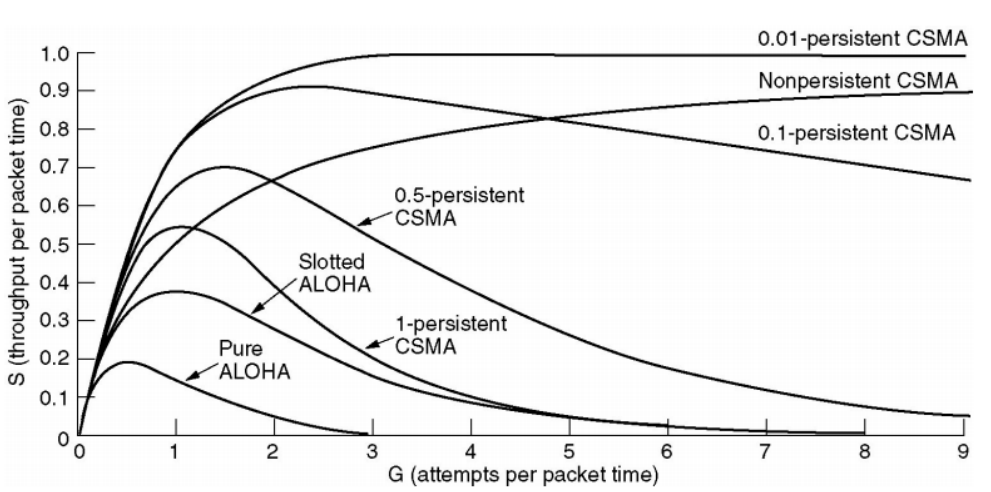
\includegraphics[width=0.7\linewidth]{MAC-G-S-graph}
\end{figure}

\subsubsection{CSMA/CD (CSMA with Collision Detection)}

\begin{outline}
	\1 Cél: ütközés érzékelése még küldés során
	\1 Ütközés esetén küldés megszakítása és:
		\2 Véletlen ideig várakozás (binary exponential backoff alapján)
		\2 "jam" jel küldése (minden állomás értesüljön az ütközésről)
		\2 16 sikertelen küldés után eldobjuk a keretet
	\1 Minimális keret méret: kétszerese annak a bájtmennyiségnek, amennyit kiküldünk az alatt az idő alatt, amíg a legtávolabbi állomás is megkapja a keretünk legelejét
		\2 Valamennyi idő kell, hogy minden állomás megkapja a keret legelejét (értesüljön, hogy küldés van folyamatban)
		\2 Ha egy állomás $\epsilon$ idővel azelőtt kezdett el küldeni, akkor még egyszer annyi idő szükséges, hogy az "eredeti" küldő is értesüljön az ütközésről
	\1 Nem szorosan kapcsolódik, de meg lett említve: maximális keret méret
		\2 MTU (Maximum Transmission Unit) általában 1500 bájt
		\2 Nagyobb keret $\implies$ nagyobb eséllyel hibás
		\2 Kisebb keret $\implies$ több keret kell $\implies$
			\3 Több bájtot pazarlunk fejlécekre
			\3 Összességében nagyobb feldolgozási idő: switch-ek csomagrátában korlátosak, csomagméret nem annyira lényeges
		\2 Adatközpontokban Jumbo keretek: pl. 9000 bájt
\end{outline}

\subsubsection{Binary Exponential Backoff (hátralék)}

\begin{outline}
	\1 Magyarul: bináris exponenciális hátralék
	\1 Cél: véletlen várakozási idő generálás ütközések számától függően
	\1 Legyen $n$ az ütközések száma (van egy számláló, felső határ: 10)
	\1 Válasszuk egy számot egyenletesen $[0;2^{n}-1]$ intervallumból
		\2 Ennyi ideig várakozzunk sikertelen küldés esetén
	\1 Az $m$-edik ütközés után átlagosan:
		\2 Sikeres átvitel esélye: $1-2^{-m}$
		\2 Átlagos késleltetés, időegységekben mérve: $\frac{1}{2} + 2^{m-1}$
	\1 Első ütközés után: 50\% siker esély, átlagosan $1,5$ rés késleltetés
	\1 Második ütközés után: 75\% siker esély, átlagosan $2,5$ rés késleltetés
\end{outline}

\pagebreak

\subsection{Ütközésmentes protokollok}

\begin{outline}
	\1 Állomások 0-tól N-ig vannak sorszámozva (előzetesen)
	\1 Réselt időmodell
\end{outline}

\subsubsection{Alapvető bittérkép protokoll}

\begin{outline}
	\1 Ütköztetési periódus, versengési időrés:
		\2 Minden állomásnak van egy időrése és vagy küld vagy nem
		\2 Így minden állomás megismeri, hogy kik és hányan akarnak küldeni
	\1 Ütköztetési periódus után adatkeretek küldése történik	
		\2 Amelyik állomás bejelentette, hogy küldeni fog, az küld
		\2 Küldési sorrend: sorszámok sorrendje
		\2 Adatkeret időrés hossza előre rögzített
	\1 Probléma: versengési időrés overhead túl nagy lehet sok állomás esetén
\end{outline}

\subsubsection{Bináris visszaszámlálás protokoll}

\begin{outline}
	\1 Egy versengési időrés és egy adatküldési időrés váltja egymást
	\1 Minden állomásnak van egy bináris azonosítója
	\1 Versengés: aki küldeni akar, elküldi az azonosítója következő bitjét
		\2 Ha bárki 1-es bitet küldött, akkor az eredmény is 1
		\2 0-t küldők kiesnek; végén egyvalaki marad, aki küldhet egy adatkeretet
	\1 Nem fair a megoldás
\end{outline}

\subsubsection{Mok és Ward bináris visszaszámlálás protokoll}

\begin{outline}
	\1 Állomások azonosítója változik (nem fix), hogy fair legyen a protokoll
	\1 Azé a legnagyobb azonosító, aki a legrégebben tudott küldeni
	\1 Aki küldött, az megkapja a minimális azonosítót
	\1 Aki akart, de nem tudott küldeni: eggyel lépteti az azonosítóját
\end{outline}

\pagebreak

\subsection{Korlátozott versenyes protokollok}

\begin{outline}
	\1 Cél: versenyhelyzetes és ütközésmentes protokollok ötvözése
	\1 Kis terhelés $\implies$ versenyhelyzetes technika (kis késleltetés érdekében)
	\1 Nagy terhelés $\implies$ ütközésmentes technika (jó kihasználtság érdekében)
\end{outline}

\subsubsection{Adaptív fabejárás}

\begin{outline}
	\1 Hasonlat: több embertől veszünk fertőzésmintát és összekeverjük a mintákat egybe, és ezt az egy nagyobb mintát teszteljük le (ami költséges)
		\2 Sok ember van letesztelve kevés költséggel
		\2 Pozitív eredmény esetén populáció felezése, tesztelés megismétlése
	\1 Időrések vannak a fa csomópontjaihoz rendelve
		\2 0. résben mindenki küldhet
		\2 Senki nem küld (üres időrés) $\implies$ figyelmen kívül hagyjuk
		\2 Ütközés van $\implies$ bal és jobb részfa megvizsgálása
		\2 Csak egyvalaki küldött $\implies$ bejárás után küldhet
	\1 Bejárás után 0, 1 vagy több állomás fog küldeni
		\2 Sorrend: bejárás sorrendje (balról jobbra)
	\1 Nagyobb terhelés $\implies$ mélyebben érdemes kezdeni a keresést	
\end{outline}

\pagebreak

\section{Adatkapcsolati réteg: legteteje, LAN, bridge}

\begin{outline}
	\1 LAN eredetileg adatszóró technológia volt
		\2 Minden adat elment minden gépbe a LAN-on (olcsó, egyszerű)
		\2 Probléma: nem skálázható, több állomás $\implies$ sok ütközés
\end{outline}

\subsection{Bridge, híd}

\begin{outline}
	\1 Több LAN összekapcsolása, de lekorlátozza az ütközési tartományokat
		\2 Plug-and-play: önmagát konfigurálja gyakorlatilag
		\2 Hurkok feloldására is képes
	\1 Hub-nál komplexebb (nem csak minden irányba ismétli a jelet)
		\2 Bridge-be ezért kell: puffer, csomag feldolgozás, routing táblák
	\1 Nem szükséges semmit módosítani a LAN-okon: ami eddig működik vagy hub-bal működne, az ezzel is fog
	\1 Switch: egyszerűsített bridge
		\2 Minden portja túloldalán csak 1 hoszt (terminál/switch) van
		\2 Így nincs szükséges CSMA/CD-re (nincs soha ütközés)
	\1 Egész internet összekötésére nem alkalmas: ismeretlen hosztot megtalálni MAC alapján, internet összes MAC címét tárolni nem reális
\end{outline}

\subsection{Keret továbbítás, MAC cím tanulás}

\begin{outline}
	\1 Minden bridge-ben van egy továbbító tábla (forwarding table)
		\2 Oszlopok: MAC cím, fizikai port, életkor
		\2 Jelentése: adott MAC cím melyik fizikai port irányában található és utoljára mikor (perc nagyságrend) adott életjelet
		\2 Régi bejegyzéseket ki lehet törölni
	\1 MAC cím tanulás
		\2 Bejövő keret forrás címét feljegyezzük a táblába
		\2 Táblát kézzel is be lehetne állítani, de akkor nem plug-and-play
	\1 Továbbító tábla alapján tudjuk, hogy egy bejövő keretet merre kell tovább küldeni (keretben benne van a címzett MAC címe)
\end{outline}

\pagebreak

\subsection{Feszítőfa protokoll (STP, Spanning Tree Protocol)}

\begin{outline}
	\1 Feszítőfa: fa, ami lefed minden csomópontot (elhagyunk éleket)
	\1 Probléma, amit megold: hurok (kör) van a hálózatban
		\2 Ilyenkor egy broadcast csomag a végtelenségig kering a hálózatban
			\3 Broadcast csomag: hálózat minden hosztjának meg kell kapnia
		\2 Több kör esetén egy broadcast csomagból akár több is keletkezhet
		\2 Jelenség neve: broadcast storm
		\2 Eredmény: előbb-utóbb a switchek túl lesznek terhelve
	\1 LAN-on általában minden link azonos (nagyságrendű) sávszélességű
		\2 Így általában nem számít, hogy melyik linket kapcsoljuk ki
		\2 De azzal, hogy kikapcsolunk linkeket, már rontjuk a hálózatban elérhető maximális sávszélességet
	\1 Terhelés eloszlással nem foglalkozik
		\2 Sőt, könnyedén kialakulhatnak hot spot-ok: forgalom jelentős része egyetlen egy ponton (switchen) megy keresztül
	\1 Feszítőfa felépítésének menete:
		\2 Egyik bridge ki van választva gyökérnek (erről később)
		\2 Minden bridge megkeresi a legrövidebb utat a gyökérhez
			\3 Felhasználható a szomszédos bridge legrövidebb út információja
		\2 Ezen legrövidebb utak uniója a feszítőfa
	\1 Felépítéshez használt üzenetek: Bridge Protocol Data Units (BPDU)
	\1 Gyökér bridge meghatározásának folyamata:
		\2 Kezdetben minden bridge azt feltételezi, hogy ő a gyökér
		\2 Bridge-ek minden irányban küldenek egy BPDU-t
		\2 Fogadott BPDU alapján minden bridge:
			\3 Gyökér frissítése: legkisebb ID-vel rendelkező
			\3 Gyökér irányába néző port frissítése
			\3 Kijelölt bridge frissítése (next hop a gyökér irányába)
	\1 Újabb alternatívák: shortest path bridging, TRILL
\end{outline}

\pagebreak

\section{Hálózati réteg (network layer)}

\subsection{Áttekintés}

\begin{outline}
	\1 Szolgáltatás: csomagtovábbítás, útvonalválasztás, fragmentálás
		\2 Csomag ütemezés (priority queueing), puffer kezelés
	\1 Interfész: csomag küldése egy adott végpontnak
	\1 Protokoll: routing táblák karbantartása, globálisan egyedi címek
	\1 Példák: IPv4, IPv6
\end{outline}

\subsection{Forgalomirányítás: útvonal meghatározás}

\begin{outline}
	\1 Feladat: bejövő csomag melyik porton legyen kiküldve (továbbítva)
	\1 Eszköz: forgalomirányító táblázat (routing table)
	\1 Elvárások: helyesség, stabilitás, igazságosság, optimalitás, hatékonyság
	\1 Algoritmus osztályok:
		\2 Adaptív: topológia és általában a forgalom is befolyásolja a döntést
			\3 Vannak különbségek ezen az osztályon belül
			\3 Honnan kapnak infót? Szomszédok? Minden router? Sehonnan?
			\3 Útvonal mikor frissül? Periodikusan? Terhelésre? Topológia?
			\3 Mit optimalizál? Távolság? Ugrások (hops)? Becsült delay?
			\3 Két fő alcsoport dinamikus algoritmusokon belül:
				\4 Távolságvektor alapú (distance vector routing)
				\4 Kapcsolatállapot alapú (link-state routing)
		\2 Nem-adaptív: offline meghatározott táblázat induláskor betöltve
	\1 Optimalitási elv: A-ból B-be vezető optimális úton elhelyezkedő routerek optimális útja B-be az előbb említett út egy része
		\2 Nyelőfa: cél a gyökér, az optimális utak a fa ágai
	\1 Feltételezés: szomszédokhoz vezető link-en lévő késleltetést valahonnan ismerjük (meg tudjuk becsülni)
\end{outline}

\pagebreak

\subsubsection{Távolságvektor alapú forgalomirányítás (distance vector routing)}

\begin{outline}
	\1 Más néven: elosztott Bellman-Ford forgalomirányítási algoritmus
	\1 Aszinkron működés
	\1 Minden állomásnak saját távolság vektora (táblázata) van
		\2 Oszlopok: hova, költség, next hop (ami általában port, router IP)
		\2 Ezt periodikusan elküldi minden direkt szomszédnak
		\2 Minden "nem ismert" állomásnak a költsége: végtelen
	\1 Kapott távolság vektor alapján frissül a saját táblázat
		\2 Frissítés: vektort küldőn keresztül költségek ellenőrzése (nőtt/csökkent)
		\2 Ha volt változás: saját táblát elküldjük minden szomszédnak egyből
	\1 Először szomszédokról van infó; fokozatosan távolabbi állomásokról is
	\1 Lassan végez az algoritmus, ha nagy a gráf átmérője
		\2 De a "jó hír" (alacsony költség) gyorsan terjed
	\1 Probléma: végtelenig számolás (count to infinity)
		\2 Fellépése: legyen 3 állomás és 2 link: A-B-C. Az A-B link megszűnik. C elküldi a táblázatát, így B azt hiszi, hogy C-n keresztül elérhető A. C megkapja B táblázatát és frissíti a saját tábláját: B-n keresztül éri el A-t, de B-ben A költsége nőtt. Ez ismétlődik végtelenségig.
		\2 Költség végtelenségig nő, a csomagok pedig ciklusban ide-oda pattognak
		\2 Megoldás: adott költség felett végtelennek tekintjük a költséget
			\3 Emlékeztető: végtelen a költsége egy nem ismert állomásnak
		\2 Hasonló probléma: link megmarad, de költsége (jelentősen) megnő
			\3 Addig nő (lassan) a költség, amíg el nem éri a valódi költséget (vagy alternatív útvonal jobb költséggel nem bír)
			\3 Azaz "rossz hír" lassan terjed
		\2 Igazi megoldás: "split horizon with poisoned reverse"
			\3 Ha az állomás X-et Y-on keresztül éri el, akkor Y-nak küldött üzenetben X költsége végtelen (negatív információ visszaküldése)
			\3 Alternatíva: csak kihagyni az üzenetből az ilyen sorokat
	\1 Egy implementáció: Routing Information Protocol (RIP)
\end{outline}

\subsubsection{Kapcsolatállapot alapú forgalomirányítás (link-state routing)}

\begin{outline}
	\1 Dijkstra algoritmusára épül
	\1 5 alapvető lépésből áll
		\2 Szomszédok keresése, hálózati címeik meghatározása (HELLO csomag)
		\2 Minden szomszédhoz költség (késleltetés) megmérése (ECHO ping)
		\2 Megismert infókból egy csomag összeállítása (pl. periodikusan)
			\3 Mezők: feladó, sorszám, korérték, szomszédokhoz költségek
		\2 Csomag elküldése az összes (nem csak a szomszédos) routernek
			\3 Csomag neve: Link State Advertisement
			\3 Küldés módja: elárasztás
		\2 Dijkstra algoritmusával: legrövidebb út számolása összes routerhez
			\3 Dijsktra működik: minden routertől kaptunk csomagot, tehát a hálózat összes router-jét és az összes link költségét ismerjük
	\1 Nagy hálózatok esetén CPU és memória igényes
	\1 Egy implementáció: OSPF (Open Shortest Path First)
		\2 Cégek és adatközpontok számára, jobban testre szabható
		\2 IPv4 felett van megvalósítva, IPv6-hoz OPSFv3 változat kell
		\2 Felépítés: átfedő területek, "Area 0" a hálózat magja
	\1 Egy implementáció: IS-IS (Intermediate System to Intermediate System)
		\2 ISP-k számára, kisebb overheaddel rendelkezik
		\2 Többfajta eszközt támogat, ami heterogén hálózatokban előny
		\2 Nem függ IP-től; IPv4 és IPv6 felett is működik
		\2 Felépítés: 2-szintű hierarchia, ahol a 2. szint a gerinchálózat
\end{outline}

\pagebreak

\subsection{Forgalomirányítás: csomag cím típusok}

\subsubsection{Unicast}

\begin{outline}
	\1 Csomag küldése két végpont között, leggyakoribb eset
	\1 Forrás és cél egyedi azonosítóval rendelkezik (IPv4, IPv6)
\end{outline}

\subsubsection{Adatszórás, broadcast}

\begin{outline}
	\1 Egy csomag egyidejűleg mindenhova elküldése
	\1 Lehetséges megvalósítások:
		\2 Külön csomag küldése minden célállomásra: sávszélesség pazarló
		\2 Elárasztás: kétpontos kommunikációhoz nem megfelelő
		\2 Többcélú forgalomirányítás (multidestination routing)
			\3 Broadcast ez egyáltalán?
			\3 Csomagban van egy címzett lista (csomópontokban módosulhat)
		\2 Forrás routerhez tartozó nyelőfa használata
			\3 Csak a feszítőfához tartozó ágakon továbbít minden router
			\3 Szükséges, hogy ismert legyen a közös feszítőfa
		\2 Visszairányú továbbítás (reverse path forwarding)
			\3 Csak akkor broadcast-oljuk a broadcast csomagot, ha az azon a linken át jött, ami az optimális next hop a broadcast csomag forrásához
	\1 Nem minden router tud minden implementációt
\end{outline}

\pagebreak

\subsubsection{Többes-küldéses forgalomirányítás, multicast}

\begin{outline}
	\1 Ugyan az az infó megy mindenhova; cél: egy link-en egyszer menjen át
		\2 Példa: IPTV szolgáltatás sávszélesség kímélő megoldása
	\1 Nem minden router támogatja
	\1 Csoport kezelés szükséges: létrehozás, megszüntetés, csatlakozás, leválasztás
		\2 Ez nem a forgalomirányítás algoritmus része
		\2 Csoport rendelkezik egy adott címmel
	\1 Minden router kiszámít egy feszítőfát, aminek azon ágain továbbítja a multicast csomagot, amelynek bármelyik pontja a csoport része
\end{outline}

\pagebreak

\subsection{Címzés: IPv4}

\subsubsection{IPv4 fejrésze}

\begin{figure}[h!]
	\centering
	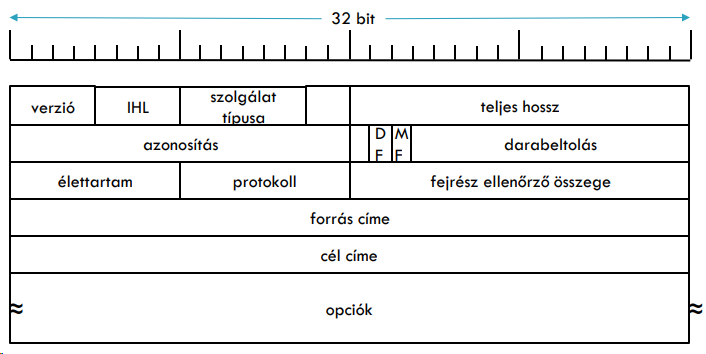
\includegraphics[width=0.8\linewidth]{ipv4-header}
\end{figure}

\begin{outline}
	\1 Verzió: IPv4 vagy IPv6
	\1 IHL: fejléc hossza 32 bites egységekben (értéke legalább 5)
	\1 Szolgálat típusa: QoS, 3 bites precedencia és 3 jelzőbit
	\1 Teljes hossz: fejléc és adatréssz együttes hossza
	\1 Azonosítás: egy datagram minden darabja azonos értéket hordozza
	\1 DF: "ne darabold" flag
	\1 MF: "több darab" flag; utolsó kivételével minden darabban "igaz"
	\1 Darabeltolás: datagramon belül ezen darab pozíciója (8 bájt egy egység)
	\1 Élettartam: minden ugrásnál eggyel csökken
	\1 Protokoll: szállítási réteg protokolljának azonosítója (pl. TCP, UDP)
	\1 Ellenőrző összeg: hibák ellen, minden ugrásnál újra kell számolni
	\1 Forrás cím, cél cím: IP címek
	\1 Opciók: opcionális (IHL megmutatja, hogy van-e), bővíthetőséget biztosít
\end{outline}

\pagebreak

\subsubsection{Lehetséges címzési struktúrák}

\begin{outline}
	\1 Sík (flat): routernek minden hoszthoz kell külön bejegyzés
		\2 pl. MAC használata, de akkor nem tudjuk sehogy se rendezni a címeket: nagyon különböző címek is tartozhatnak azonos alhálóba
		\2 Eredmény: túl nagy routing táblák, amik nehezen karbantarthatók
	\1 Hierarchikus: címek konkrét területet leíró szegmensekből állnak
		\2 Hasonló a telefonszámokhoz
		\2 Ha változik a cím, akkor nem kell minden router-t frissíteni: pl. ha a cím legvége változott, akkor elég az utolsó router-t frissíteni
\end{outline}

\subsubsection{IP cím}

\begin{outline}
	\1 Minden hoszt és router rendelkezik egyedi, 4 bájtos címmel
	\1 Réges régen 5 címosztály lett definiálva: A, B, C, D, E
		\2 A: '0' + 7 bit hálózat + 24 bit hoszt
		\2 B: '10' + 14 bit hálózat + 16 bit hoszt
		\2 C: '110' + 21 bit hálózat + 8 bit hoszt
		\2 D: '1110' + ...: többesküldéses cím
		\2 E: '1111' + ...: jövőbeli felhasználás
		\2 Előny: alhálózati maszk nem kell, mert a cím struktúrája kódolja
	\1 Hoszt és hálózat elkülönítése mögötti motiváció: hoszt bitekkel csak a hálózaton belül kell foglalkozni; kisebb routing táblákkal lehet dolgozni
	\1 Speciális címek:
		\2 0.0.X.Y: egy hoszt a helyi hálózaton
		\2 255.255.255.255: adatszórás helyi hálózaton
		\2 X.Y.255.255: adatszórás egy adott hálózaton
		\2 127.X.Y.Z: visszacsatolás (loopback; bitek: 0, 7db 1, utána bármi)
	\1 Alhálózatok: alhálózati maszk (subnet mask) alapján, pl. 172.15.223.0/24
		\2 Egy router egy 24 bites hoszt cím tartományt nem tud kezelni
		\2 Táblázatban (hálózat,0) és (saját hálózat, hoszt) típusú bejegyzések
		\2 Nincs találat $\implies$ alapértelmezett router felé továbbítás
\end{outline}

\pagebreak

\subsubsection{CIDR}

\begin{outline}
	\1 Motiváció: cím osztályok nem praktikusak, mert a B címek gyorsan elfogytak, C címek pedig túl kevés hosztot tartalmazhatnak
	\1 C osztályos címtartományok egy csoportját kapják az igénylők
	\1 Forgalomirányítás bonyolódik:
		\2 Szükség van 32 bites alhálózati maszkra
		\2 Routing táblában innentől ilyen egy sor:\\
		IP cím, alhálózati maszk, következő ugrás
		\2 Cím alhálózat része alapján, a leghosszabban illeszkedő tábla bejegyzés alapján route-olunk
	\1 Túl sok routing tábla bejegyzésre megoldás:
		\2 Aggregálás, azaz csoportos bejegyzések
		\2 Azonos next hop esetén elég a címek egyező kezdőszeletét tárolni
\end{outline}

\subsection{NAT (Network Address Translation, hálózati címfordítás)}

\begin{outline}
	\1 Gyors javítás IP címek elfogyása ellen
	\1 Háztartásonként/cégenként elég egy globális IP cím, a hálózaton belül pedig minden gép egy másik címtartományból kap egyedi címet
		\2 Belső hálózat határán átmenő csomagok esetén címfordítás kell
		\2 Belső címtartományokhoz ezek vannak lefoglalva:\\
		10.0.0.0/8 és 172.16.0.0/12 és 192.168.0.0/16
	\1 Címfordítás működése
		\2 Szállítási réteget is használja: UDP/TCP port mezőket használja
		\2 Kimenő csomagnál elmentjük, hogy a forrás port melyik belső IP címhez tartozik és egy új, egyedi forrás portra cseréljük
	\1 Problémák:
		\2 Szállítási réteghez (TCP, UDP) szorosan hozzá van kötve
		\2 Csak 65536 lehetséges port van, ez nem feltétlenül elég
\end{outline}

\pagebreak

\subsection{MTU és IP fragmentation (darabolás, fragmentáció)}

\begin{outline}
	\1 MTU: Maximum Transmission Unit
		\2 Minden hálózatnak (routernek) lehet saját MTU értéke
		\2 Gyakorlatban majdnem minden hálózatban 1500 bájt
	\1 Ha egy csomag túllépi az MTU-t, akkor el lehet dobni
		\2 Meg van engedve: az IP csak "best effort delivery"-t ígér
		\2 Problémás, pl. VPN esetén: ami eredetileg MTU alatti csomagméret volt, a VPN extra fejlécek miatt már lehet túl nagy
	\1 IPv4: ha egy csomag túllépi az MTU-t, akkor szét lehet vágni
		\2 IPv6-ban ilyen nincsen alapból (de MTU és MTU discovery van)
		\2 IPv4 fejléc második 32 bitje ehhez kapcsolódik
			\2 Eredeti csomaghoz azonosító, darabkák öröklik
				\3 "flow id"-val közösen egyedi azonosítót alkot
				\3 Flow-on belüli párhuzamosan több csomag lehet így fragmentálva
			\2 Flags: "reserved", "don't fragment" és "more fragments"
				\3 "more fragments" jelentése: ez nem az utolsó darab
			\2 Fragment offset: a darabkra a payload melyik részét tárolja
		\2 Akkor sikeres egy továbbküldés, ha minden kis darabka átment
			\3 Ha csak egy is elveszik, akkor az összes haszontalan
			\3 Ezért nem érdemes túllépni az MTU-t küldésnél
		\2 Egy csomag többször is szétvágható
		\2 Csomag összerakás: fogadó állomásnál
		\2 Kihívások fogadó félnél (mert nincs végtelen memória: puffer véges)
			\3 Darabok nem sorrendben érkeznek
			\3 Duplikáltan érkezhet meg darab
			\3 Darab hiányzik, nem érkezik meg
		\2 Problémás eset: virtualizáció van és a CPU-nak kell rengeteg csomagot fragmentálni
	\1 IPv4/6-ban van MTU discovery protocol: "can't fragment" router válasz
		\2 Primitív megoldás: "don't fragment" bitű csomag küldése csökkenő mérettel, amíg válasz nem jön
\end{outline}

\pagebreak

\subsection{IPv6}

\begin{outline}
	\1 Motiváció: kevés az IPv4 cím
	\1 Megoldás: 32 bit helyett 128 bites címek
		\2 Formátum: 8 darab 16 bites hex csoport, elválasztó: "\texttt{:}"
		\2 Csoportokban a prefix "0"-k elhagyhatók
		\2 Egy helyen \texttt{a:0:0:...:0:b} helyettesíthető \texttt{a::b}-vel
	\1 Localhost: \texttt{::1}
	\1 Címkiosztás:
		\2 Általában 64 bites alhálózat címtartományok vannak kiosztva
		\2 CIDR-ről már nem beszélünk, de router-ben aggregáció használt
	\1 Teljesítmény növekedés:
		\2 Fejlécben nincsen checksum, amit számolni kéne
		\2 Egyszerűbb routing tábla szerkezet
		\2 Nincs szükség fragmentáció kezelésre
\end{outline}

\subsubsection{IPv6 fejléc}

\begin{figure}[h!]
	\centering
	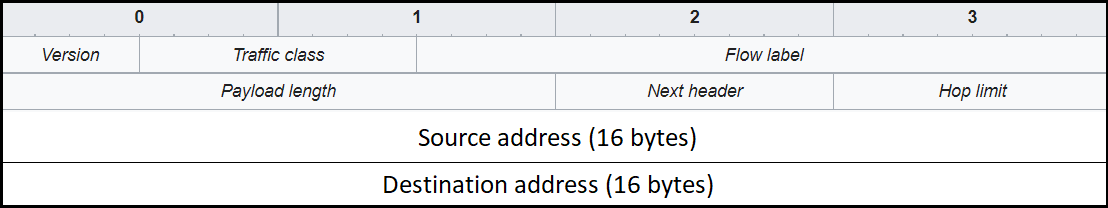
\includegraphics[width=1\linewidth]{ipv6-header}
\end{figure}


\begin{outline}
	\1 20 bájtos IPv4 fejléc helyett 40 bájt
	\1 IPv4-ben is volt: verzió és DSCP/ECN (QoS)
	\1 Flow label: adatfolyam azonosító
	\1 Next header: mint IPv4-ben a protokoll mező (következő fejléc típusa)
	\1 Hop limit: mint IPv4-ben a TTL (csak át lett nevezve)
\end{outline}

\pagebreak

\subsubsection{További IPv6 lehetőségek}

\begin{outline}
	\1 Source routing (forrás routing): küldő határozza meg a csomag útvonalát
	\1 Mobil IP: állomás magával viszi az IP címét másik hálózatba
		\2 Szólni kell az eredeti hálózat routerének, hogy most máshová mentem
		\2 Source routing-ot használ
	\1 Privacy kiterjesztések: véletlenszerűen generált állomás azonosító
	\1 Jumbogram: 4Gb-es datagram támogatás
\end{outline}

\subsubsection{Bevezetésnek nehézségei}

\begin{outline}
	\1 1998-ban mutatták be az IPv6-ot, miért van még mindig IPv4?
	\1 Ez a réteg felelős a globális konnektivitásért, itt homogenitás kell
	\1 Minden router-nek, minden hosztnak kéne IPv6-ot támogatni
		\2 Hosztok (Windows, Android) és otthoni router-ek már támogatják
		\2 Gerinchálózatra (nagy, gyors, drága eszközök) várunk elsősorban
	\1 Több protokollt is meg kell valósítani IPv6-ra (pl. ICMPv6, DHCPv6)
	\1 Egy megoldás: IPv6 csomagokat tunnel-el becsomagolni IPv4-be
\end{outline}

\pagebreak

\subsection{Forgalom irányítás az interneten}

\begin{outline}
	\1 Hálózati rétegben az internet autonóm rendszerek összekapcsolt együttese
		\2 Vannak gerinchálózatok, regionális hálók, vállalati hálók, stb.
		\2 Azaz többszintű routing-ról beszélünk, de mindegyik IP-t használ
			\3 Pl. vállalati háló használ spanning tree-t, gerincháló nem
		\2 LAN-on belül a routereket az adatkapcsolati réteg kapcsolja össze
	\1 Két szintű hierarchia:
		\2 Autonóm rendszerek belsejei
		\2 Autonóm rendszerek összekapcsolva, ezek összessége
\end{outline}

\subsubsection{Autonóm rendszer, Autonomous system, AS}

\begin{outline}
	\1 Példa: Verizon, Telekom, ELTE
	\1 Motiváció, miért van rájuk szükség
		\2 Eddig tanult routing algoritmusok nem elég hatékonyak, hogy az internet teljességén működjenek (megoldás: BGP)
		\2 Más szervezetek más forgalomirányítási policy-t akarnak
		\2 Lehetőséget ad a belső hálózat szerkezetének elrejtésére
		\2 Lehetőség a szervezetnek eldönteni, hogy merre irányítása a saját forgalmát és másik irányíthassa-e rajta keresztül
	\1 Minden AS-t egy ASN azonosít (eredetileg 16 bit, most már 32)
	\1 AS-k szélen olyan routerek kellenek, amik inter- és intra-domain routingot is tudnak
	\1 Hálózatok csoportosítása:
		\2 Csonka (stub): egyetlen összeköttetés a BGP gráffal
		\2 Többszörösen bekötött (multihomed): több BGP router is van, de nincs átmenő forgalom
			\3 pl. adatközpontok: redundáns bekötés a cél
		\2 Tranzit (transit): fizetés ellenében harmadik fél csomagjait továbbítják
		\2 IXP, Internet eXchange Point: sok AS közvetlen összekötése
\end{outline}

\pagebreak

\subsubsection{Intra-domain routing (AS-en belül)}

\begin{outline}
	\1 Pl. Routing Information Protocol
	\1 Pl. Open Shortest Path First
\end{outline}

\subsubsection{Inter-domain routing (AS-ek között)}

\begin{outline}
	\1 Protokoll: BGP-4 (Border Gateway Protocol), nincs másik
		\2 Homogenitás szükséges, hogy globális konnektivitás legyen
		\2 Verziók visszafelé kompatibilisek
		\2 TCP-t használ a BGP a kommunikációhoz
	\1 Tulajdonságok
		\2 Jól skálázható és rugalmas útvonal választás
		\2 Konfigurálható az útvonal, pl. adott AS-ek, vagy országok kizárása
	\1 AS-ek hierarchiája
		\2 Peering link: egyenrangú AS-ek között (pl. két Tier-1 ISP között)
			\3 Csak olyan forgalom mehet át, ami a link egyik végén keletkezett és a másik végén terminál
			\3 Indoklás: más forgalomból az összekötő AS-nek nincs bevétele
		\2 Transit link: eltérő rangúak között (pl. ISP és végfelhasználó)
			\3 Az alacsonyabb rangú fizet a magasabb rangúnak a használatért
		\2 Egy Tier-1 ISP-nek nincsen szolgáltatója, ő a csúcs, ő minden másik Tier-1 ISP-vel peering agreement-ben van
\pagebreak
	\1 BGP működése: path vector routing (útvonal vektor routing)
		\2 Distance vector kiterjesztése: teljes útvonal számon van tartva
			\3 Nincs végtelenig számolás probléma
			\3 Hirdetés során is a teljes útvonalak vannak átadva
		\2 Longest Prefix Match alapján van az útvonal kiválasztva
		\2 Saját útvonal választási politika alkalmazható
			\3 Útvonal kiválasztás: melyik útvonal legyen használva?
			\3 Útvonal export: melyik útvonal legyen meghirdetve valakinek?
			\3 Peering szerződés is ilyen módon van megoldva
		\2 Példa routing mintára: hot potato routing: csomagot lehető leggyorsabban átadjuk másik AS-nek, akkor is, ha a miénkben több ideig maradna, akkor gyorsabban célba érhetne
		\2 Egy ISP milyen route-okat importál, exportál?
			\3 Importálás: customer, peer, provider összes route-ja
			\3 Exportálás customer felé: összes route
			\3 Exportálás peer és provider felé: customer route-jai
				\4 Ha peer-be megy a route, akkor peer felé van exportálva
	\1 BGP elnevezése/változatai felhasználástól függően:
		\2 eBGP, External BGP: routing információk cseréje AS-ek között
		\2 IGP, Interior Gateway Protocol: útválasztás AS-en belüli célállomáshoz
			\3 Ez nem BGP, hanem pl. OSPF, IS-IS
		\2 iBGP, Internal BGP: útválasztás egy AS-en belül egy külső célállomáshoz
		\2 Példa működésre:
			\3 eBGP segítségével a határ router megismeri az útvonalat egy külső célállomáshoz
			\3 iBGP segítségével a AS többi routere is megismeri ezt az útvonalat (de valahogy el kell jutni a határ routerig először)
			\3 IGP segítségével egy csomag eljuttatható AS-en belül bárhova, a határ routerig például
\end{outline}

\pagebreak

\section{Logikailag hálózati réteghez tartozó protokollok}

\subsection{ICMP, Internet Control Message Protocol}

\begin{outline}
	\1 Feladat: váratlan események jelentése
	\1 Pár lehetséges üzenet és azok lehetséges okai:
		\2 Elérhetetlen cél: csomag kézbesítése nem sikerült
			\3 Lehetséges ok: nem darabolható csomag túllépte az MTU-t
		\2 Időtúllépés: csomag élettartam mezője elérte a 0-t
			\3 Lehetséges ok: hurok alakult ki pl. torlódás miatt
			\3 Lehetséges ok: számláló kezdeti értéke túl kevés volt
		\2 Paraméter probléma: fejrészben érvénytelen mező
			\3 Lehetséges ok: router vagy hoszt szoftver hiba
		\2 Forráslefojtás: egy fél küldheti, ilyenkor a fogadó állomásnak a forgalmazást lassítania kell
		\2 Visszhang kérés: ping parancs, a fogadó válaszol
		\2 Átirányítás: csomag rosszul irányítottságát jelzi
			\3 Lehetséges ok: nem optimális útvonalon jött a csomag
\end{outline}

\subsection{ARP, Address Resolution Protocol}

\begin{outline}
	\1 Feladat: IP cím megfeleltetése egy fizikai címnek
		\2 Adatkapcsolati és hálózati réteg összekapcsolása menedzsment szinten
		\2 LAN-on belül értelmes: csak LAN-on belüli címzéshez kell MAC
	\1 Hozzárendelés menete:
		\2 Adatszóró csomag küldése Ethernet-re: "Kié a X.Y.Z.W IP cím?"
		\2 Hosztok összehasonlítják a kapott és a saját IP címüket
		\2 Egyezés esetén a hoszt válaszol a saját MAC címével
	\1 Cache-eléssel hatékonyabbá tehető: IP-MAC cím párok elmenthetők
		\2 Timeout-ot szokás használni: így az IP-hez rendelt MAC megváltozhat
	\1 Távoli hálózaton található hoszt kezelése
		\2 Router válaszol az ARP kérésekre (proxy ARP)
		\2 Összes távoli forgalomhoz az alapértelmezett Ethernet-cím használata
\end{outline}

\pagebreak

\subsection{RARP, Reverse Address Resolution Protocol}

\begin{outline}
	\1 Feladat: fizikai cím megfeleltetése egy IP címnek
	\1 Hozzárendelés menete:
		\2 Adatszóró csomag küldése Ethernet-re: "Az N bites fizikai címem F, mi az IP címem?"
			\3 Gyakorlatban mindig 48 bites MAC cím a fizikai cím
		\2 RARP szerver válaszol a megfelelő IP címmel
	\1 Alternatívák, javítási lehetőségek:
		\2 BOOTP protokoll: statikus címkiosztás UDP használatával
		\2 DHCP protokoll: lásd lejjebb
\end{outline}

\subsection{DHCP, Dynamic Host Configuration Protocol}

\begin{outline}
	\1 Feladat: fizikai cím alapján a kommunikációhoz szükséges adatok átadása
		\2 Eredetileg a BOOTP kiterjesztése volt
	\1 Kiszolgáló és kérő állomás más LAN-on is lehet, viszont ekkor a LAN-ban kell egy DHCP relay agent
	\1 DHCP lehetőségei
		\2 Statikus címkiosztás: adott MAC mindig ugyan azt az IP-t kapja
		\2 Dinamikus címkiosztás: IP tartományból érkezési sorrendben kapnak
			\3 Ilyenkor elég akkora tartomány, ahány kliens egyidejűleg működik
		\2 Hálózati paraméterek átadása: hálózati maszk, alapértelmezett átjáró, névkiszolgáló, stb.
	\1 Címek bérlése
		\2 Egy kliens csak egy adott ideig kap meg egy IP-t (lease time)
			\3 Kliens kérése tartalmazhatja, hogy ő mennyi időt szeretne
			\3 Szerver konfigurációja a kliens kérését felülírhatja
		\2 Lejárat előtt a bérlést meghosszabbíthatja a kliens
		\2 Az IP cím explicit módon vissza is adható
\end{outline}

\pagebreak

\subsection{VPN, virtuális magánhálózatok}

\begin{outline}
	\1 Feladat, megoldandó probléma:
		\2 Probléma: cégnek több telephelye van vagy lehet otthonról dolgozni
		\2 Cél: cégnek egy nagy privát hálózata legyen (logikailag)
		\2 Régi megoldás: dedikált vonal vásárlása telephelyek között
	\1 Működés: bérelt vonal helyett virtuális linkek
		\2 Virtuális linkek interneten átmenő alagutakkal vannak megvalósítva
		\2 Alagút endpoint lehet a LAN-ban lévő router vagy a kliens számítógép
		\2 Alagútba belépéskor a csomag egy másik csomagba kerül beágyazásra
			\3 Megnevezése: IP az IP-be mechanizmus
	\1 Autentikáció, titkosítás: IPSEC segítségével
		\2 Autentikáció: ne tudjon bárki VPN-hez csatlakozni
		\2 Titkosítás: az alagútban lévő csomagok titkosítva legyenek
\end{outline}

\subsubsection{IPSEC}

\begin{outline}
	\1 Hosszú távú cél: biztonságos IP réteg
	\1 Műveletek, mit foglal magába:
		\2 Hoszt párok kommunikációjához kulcsok biztosítása
		\2 Kommunikáció kapcsolatorientáltabbá tétele
		\2 Fejlécek és láblécek hozzáadása az IP csomagok védelme érdekében
	\1 Több módot támogat, ezek egyike az alagút mód
		\2 ESP header: Encapsulating Security Payload
		\2 HMAC: Hash-based Message Authentication Code
\end{outline}

\pagebreak

\section{Szállítói réteg (transport layer)}

\begin{outline}
	\1 Szolgáltatás: multiplexálás, megbízhatóság, sorrendhelyesség
		\2 Torlódásvezérlés: enélkül újraküldések miatt telítődne a puffer
		\2 Fairség és csatorna kihasználtság egyensúlyozása
		\2 Hosszú élettartamú kapcsolatok támogatása
	\1 Interfész: üzenet küldése cél processznek
	\1 Protokoll: port szám, folyamfelügyelet, megbízhatóság
	\1 Példa: UDP, TCP
\end{outline}

\subsection{Multiplexálás}

\begin{outline}
	\1 Egy kliens számos alkalmazást futtathat egy időben
		\2 Másik eset: egy szerver számos klienssel beszél egyszerre
	\1 El kell dönteni, hogy egy adott csomag melyikhez tartozik
	\1 IP fejléc protokoll mezője 8 bites, ez nem elég nagy
	\1 Megoldás: portok bevezetése
\end{outline}

\subsection{Réteg modellek áttekintés}

\begin{outline}
	\1 Alacsonyabb rétegekben (fizikai, adatkapcsolati, hálózati) a szomszéd hosztokkal kommunikálnak az eszközök
	\1 Szállítói (és alkalmazási) réteg: közvetlenül a cél hoszttal kommunikálunk
		\2 Peer-to-peer kommunikáció: gyakorlatilag a cél lett a szomszédunk
		\2 Szállítói réteg fejléceit csak a forrás és cél végpontok olvassák ki
			\3 Nem teljesen igaz: pl. tűzfal vagy DDoS védelem miatt routerek is sokszor megnézik az UDP/TCP fejléceket
\end{outline}

\pagebreak

\subsection{UDP}

\begin{figure}[h!]
	\centering
	\includegraphics[width=0.7\linewidth]{"udp-header"}
\end{figure}

\begin{outline}
	\1 Egyszerű, kapcsolat nélküli átvitel
	\1 Kicsi, 8 bájtos fejléc
		\2 Demultiplexálás portszámok segítségével
			\3 16 bites port, 0-ás port nem megengedett $\to$ 65535 lehetőség
		\2 Kontrollösszeg segítségével hibás csomagok felismerhetőek
			\3 Nincs védelem elveszett, duplikált és helytelen sorrendben érkező csomagoktól
	\1 Motiváció (TCP után vezették be)
		\2 TCP nem minden alkalmazásnak megfelelő
		\2 UDP felett egyedi protokollok valósíthatóak meg
			\3 Megbízhatóság, helyes sorrend nem mindenkinek szükséges
				\4 pl. real-time média streamelés megfelelő enkódolással
			\3 Adatközpontokban saját folyamvezérlés protokollok alkalmazása
\end{outline}

\subsection{TCP}

\begin{figure}[h!]
	\centering
	\includegraphics[width=0.7\linewidth]{"tcp-header"}
\end{figure}

\begin{outline}
	\1 TCP egy absztrakt bájt folyam megvalósítása
	\1 Megbízható, sorrend helyes, kapcsolat alapú két irányú bájt folyam
	\1 20 bájtos fejléc + options fejlécek (UDP-vel azonos port rendszer)
	\1 TCP-ben van: folyam vezérlés, torlódás vezérlés, fair csatorna hozzáférés
\end{outline}

\pagebreak

\subsubsection{Kapcsolat kezelés}

\begin{outline}
	\1 Miért szükséges? Miért kapcsolat-alapú a TCP?
		\2 Állapot kialakítása mindkét végponton
		\2 Példa: sorszámok (sequence numbers) számontartása
	\1 Pár fontos TCP flag (1 bites jelölő):
		\2 SYN: szinkronizációs, kapcsolat felépítéshez
		\2 ACK: fogadott adat nyugtázása
		\2 FIN: vége, kapcsolat lezáráshoz
	\1 Kapcsolat felépítése: three way handshake (három-utas kézfogás)
		\2 Cél: mindkét fél ismerje meg a másik fél kezdő sorszámát és mindkét fél nyugtázza a másik fél kezdő sorszámát
		\2 Első lépés: kliens $\to$ szerver: [SYN, SeqK, 0]
		\2 Második lépés: szerver $\to$ kliens: [SYN/ACK, SeqS, SeqK+1]
		\2 Harmadik lépés: kliens $\to$ szerver: [ACK, SeqK+1, SeqS+1]
			\3 Ebben az üzenetben már payload is lehet
		\2 Támadási felület: minden SYN állapotot foglal a szerveren
			\3 SYN flood, DoS egy fajtája: csak SYN küldése, de belőle sok
			\3 Megoldás a SYN cookies: kezdeti sorszámba enkódolja a tárolandó állapotot ahelyett, hogy az első SYN-nél letárolná a szerver
	\1 Kapcsolat lezárása
		\2 Bármely oldal kezdeményezheti a lezárást
		\2 Menete: FIN flag küldése, majd másik fél is küld FIN-t
			\3 FIN-t tartalmazó csomagokat is nyugtázni kell
		\2 Kihívás: egyik fél lezárta, de másik fél még küld újabb csomagot
		\2 Félig nyitott kapcsolat: egyik fél lezárta, másik még nem
\end{outline}

\pagebreak

\subsubsection{Sorszámok}

\begin{outline}
	\1 Minden bájtnak van egyedi sorszáma: 32 bites érték, idő után körbefordul
		\2 Kezdeti sorszám biztonsági okokból véletlen szám: nehéz kitalálni
	\1 Bájt folyam szegmensekre (TCP csomagokra) van bontva
		\2 Maximális méret: MSS (Maximum Segment Size)
		\2 MSS-t úgy kell beállítani, hogy ne legyen fragmentáció
		\2 Szegmenseknek van egyedi sorszámuk: első bájt sorszáma
	\1 Két irányba két különböző sorszám létezik
		\2 Hiszen mindkét fél küldhet és fogadhat is adatot, akár párhuzamosan
\end{outline}

\subsubsection{Folyamvezérlés}

\begin{outline}
	\1 Probléma: küldő milyen gyorsan küldheti az adatot?
		\2 Túl sok csomag túlterheli a fogadót
		\2 Fogadó oldal puffer mérete változhat a kapcsolat során
			\3 Ez a puffer az (app általi) feldolgozásra váró bájtokat tárolja
	\1 Megoldás: csúszóablak (sliding window)
		\2 Fogadó megosztja a pufferének a méretét (ez az advertised window)
			\3 Magyarul meghirdetett ablak, és értéke akár 0 is lehet
		\2 Küldő $N$ ablakméretnél $N$ bájtot küldhet nyugta fogadása nélkül
		\2 Csúszóablak előre lép (csúszik) minden nyugta fogadásakor
		\2 Átvitel, átvitt adatmennyiség $\sim \frac{\text{w (window)}}{\text{RTT (Round Trip Time)}} = \frac{\text{küldési ablakméret}}{\text{körülfordulási idő}}$
			\3 Rövid RTT $\implies$ ACK gyorsan jön $\implies$ ablak gyorsan lép
\end{outline}

\begin{figure}[h!]
	\centering
	\includegraphics[width=0.65\linewidth]{"csúszóablak"}
\end{figure}

\pagebreak

\begin{outline}
	\1 Nyugtázás típusok
		\2 Minden csomag külön nyugtázása
		\2 Kumulált nyugta: minden $K<N$ sorszámú csomag nyugtázása
			\3 TCP-ben alapértelmezett, de nem ez a leggyakoribb
		\2 Negatív nyugta (NACK): adott csomag hiányának jelzése
		\2 Szelektív nyugta (SACK): megérkezett csomagot felsorolása
			\3 Nem az alap TCP része: SACK TCP nevű kiterjesztés
			\3 Gyakorlatilag minden TCP implementáció ezt használja
			\3 Felesleges újraküldések számát jelentősen csökkenti
	\1 Túl kicsi ablak $\implies$ sok kicsi csomag, fejlécek dominálják az átvitelt
	\1 Nagle algoritmusa: kicsi csomagok küldésének elkerülése
		\2 Cél: ne pazaroljuk a sávszélességet fejlécekkel, stb.
		\2 Ha ablak $>=$ MSS és elérhető adat $>=$ MSS: küldés
		\2 Különben ha van nem nyugtázott adat: várakozás nyugtára/adatra
		\2 Különben: "nem teljesen telített" csomag küldése
		\2 Probléma: késleltetve van az átvitel
			\3 Használható \texttt{TCP\_NODELAY} flag, ha azonnali küldés szükséges
\end{outline}

\subsubsection{(Sorrend/kontrollösszeg) hiba detektálás, újraküldés}

\begin{outline}
	\1 Fogadó oldal:
		\2 Kontrollösszeg újraszámolása és összehasonlítása a fejlécbeli értékkel
			\3 A kontrollösszeg az IP, TCP fejlécből és az adatból van számolva
			\3 Hibás kontrollösszeg esetén a csomagot eldobjuk
		\2 Sorszámok segítségével sorrendhelyes átvitel garantálása
			\3 Duplikátumok eldobása
			\3 Helytelen sorrendben érkező csomagok sorba rendezése / eldobása
				\4 Fogadhatunk nem sorrendhelyesen, ha a pufferbe befér
			\3 Hiányzó sorszámok elveszett csomagot jeleznek
	\1 Küldő oldal:
		\2 Minden nyugtázatlan csomag pufferelése a nyugta megérkezéséig
		\2 Időtúllépés (timeout) segítségével hiányzó nyugták érzékelése
\end{outline}

\pagebreak

\begin{outline}
	\1 Időtúllépés újraküldéshez (RTO, Retransmission Time Outs)
		\2 RTO az RTT-től függ: ennyi idő alatt ér vissza ideálisan a nyugta
		\2 TCP-ben RTT becslése: mozgó átlaggal
			\3 \texttt{new\_rtt = a * old\_rtt + (1-a) * new\_sample}
			\3 \texttt{new\_sample} egy küldés és az ACK megérkezés közötti idő
			\3 Minden küldés-nyugta párnál frissítjük az értéket
				\4 Karn algoritmusaa: eldobjuk azokat a mintákat, melyek egy újraküldésből származnak
				\4 Indoklás: Mi van, ha nagyon megugrott az RTT, és közvetlenül az újraküldés után megérkezik az eredeti nyugta?
			\3 \texttt{a} javasolt értéke: $0.8$ és $0.9$ között (általában $0.875$)
		\2 \texttt{RTO = 2 * new\_rtt} (konzervatív becslés, internetre egész jó)
			\3 RTO alsó korlát: 300ms, ami adatközpontokban problémás (hiszen RTT $\approx$ 1ms), lásd pl. TCP incast problem
\end{outline}

\subsubsection{Torlódás bevezetés}

\begin{outline}
	\1 Torlódás akkor van, ha a hálózat terhelése nagyobb, mint a kapacitása
	\1 Torlódás fellépésnek lehetséges okai:
		\2 Hálózatban a kapacitás nem egyenletes, pl. modem vs üvegszál
		\2 Több folyam verseng a sávszélességért, pl. filmnézés és böngészés
		\2 Időben egyenletlen a terhelés, pl. GoT-t mindenki egyszerre nézi
	\1 Torlódás következménye: csomagvesztés
		\2 Router gyorsabban kap csomagokat, mint ahogy küldeni tud
		\2 Router véges pufferrel rendelkezik $\implies$ el kell dobni csomagokat
		\2 RED (Random Early Detection): ahogy telítődik a puffer, úgy nagyobb eséllyel dobjunk el véletlenszerűen csomagokat
	\1 Csomagvesztés következménye:
		\2 Megnövekedett késleltetés (mert csomagok újraküldése szükséges)
			\3 Egyébként is nő: puffer végére kerül az új csomag, várnia kell
		\2 Sávszélesség pazarlás újraküldések miatt
		\2 Alacsony hálózati átvitel a pazarlások miatt (goodput)
\end{outline}

\pagebreak

\begin{figure}[h!]
	\centering
	\includegraphics[width=0.65\linewidth]{"terhelés"}
\end{figure}

\begin{outline}
	\1 Könyök (knee) után: átvitel alig, késleltetés gyorsan nő
	\1 Szírt (cliff) után: átvitel $\to 0$, késleltetés $\to \infty$ (teljes összeomlás)
	\1 Késleltetés egyszerűsített modellezése: késleltetés $\sim \frac{1}{1 - \text{utilization}}$
	\1 Torlódás elkerülés: könyök bal oldalán maradás
	\1 Torlódás vezérlés: szírt bal oldalán maradás
\end{outline}

\subsubsection{Torlódás vezérlés (congestion control)}

\begin{outline}
	\1 TCP-nek alapból nem volt része, de később szükségessé vált
	\1 Valójában torlódás elkerülést végez a TCP (könyök közelítése a cél)
	\1 Konstans méretű ablak csak a fogadót védi a túlterheléstől
		\2 Nem segít, ha a hálózat a szűk keresztmetszet és nem a fogadó
		\2 Megoldás: állítható ablakmérettel a küldési ráta korlátozása
	\1 Általános megoldási lehetőségek
		\2 Ne csináljunk torlódás vezérlést
			\3 Jósolhatatlan teljesítmény, akár teljes összeomlás
		\2 Erőforrás foglalás
			\3 Küldés előtt folyamokhoz előre sávszélességet foglalunk
			\3 Hálózati támogatás szükséges
		\2 Dinamikus beállítás (TCP ezt csinálja)
			\3 Torlódási szint becslése, ez alapján küldési ráta csökkentése/növelése
			\3 Elosztott koordináció, nem rendezett dinamika
\end{outline}

\pagebreak

\begin{outline}
	\1 Küldő oldalon torlódási ablak bevezetése (cwnd, congestion window)
		\2 Cél: ablak méretének változtatása küldési ráta változtatásához
		\2 Hiszen a küldési ráta arányos a $\frac{\text{window}}{\text{RTT}}$ értékével
		\2 \texttt{window = min(congestion\_window, advertised\_window)}
	\1 Torlódás detektálás
		\2 Késleltetés alapú megoldások nehezek és kockázatosak, pontatlanok
		\2 Eldobott csomag egy biztos jel
			\3 Időkorlát lejárt és nem jött nyugta $\implies$ csomagvesztés történt
			\3 Számos duplikált ACK jön sorban $\implies$ csomagvesztés történt
				\4 Duplikált nyugtákról, e mögötti logikáról később lesz szó
	\1 Általános algoritmus
		\2 ACK jött $\implies$ cwnd növelése
			\3 Adat sikeresen átment, tehát valószínűleg gyorsabban is küldhetünk
			\3 Következmény: RTT-től függ a növelések gyakorisága
		\2 Csomagvesztés történt $\implies$ cwnd csökkentése
			\3 Adat elveszett, tehát valószínűleg torlódás van
		\2 Implementáció feladata: cwnd növelés/csökkentés mit jelent pontosan
	\1 TCP Tahoe: TCP-ben az eredeti algoritmus implementáció
		\2 \texttt{ssthresh}: könyökpont alsó becslés, alapból \texttt{ssthresh = advertised\_window}
		\2 Slow start, lassú indulás fázis: cwnd $<$ ssthresh és nincs csomagvesztés
			\3 Cél: (ismeretlen "értékű") könyökpont (bottleneck) gyors elérése
			\3 Indulás: \texttt{cwnd = 1}
			\3 Minden nyugtázott szegmens esetén cwnd növelése eggyel
				\4 Tehát cwnd időben exponenciálisan nő: RTT-nként duplázódik
		\2 Torlódás elkerülés fázis: cwnd $>=$ ssthresh
			\3 AIMD: Additive Increase Multiplicative Decrease
				\4 TCP Tahoe valójában még nem multiplicative decrease
			\3 Nyugtázott szegmens esetén \texttt{cwnd += 1/cwnd}
				\4 Tehát cwnd időben lineárisan nő: kb. RTT-nként eggyel
			\3 Csomagvesztés esetén: induljon egy slow start fázis elölről \texttt{ssthresh := cwnd / 2} értékkel
		\2 Ez az algoritmus működik, de nem túl hatékony, hamar lecserélték
\end{outline}

\pagebreak

\begin{outline}
	\1 TCP Reno: TCP Tahoe kiegészítése
		\2 Gyors újraküldés: 3 duplikált ACK $\implies$ újraküldés, ne várjunk
			\3 Alapból meg kéne várni az RTO-t
			\3 Ha több küldött csomagból az első elveszik, akkor a fogadó az elveszett előttihez tartozó ACK-t küldi minden megérkezetthez
		\2 Gyors helyreállítás: gyors újraküldéskor \texttt{ssthresh:=cwnd:=cwnd/2}
			\3 Ezzel a felesleges slow start fázis el van kerülve
			\3 RTO lejárta esetén továbbra is \texttt{cwnd:=1} van érvényben
				\4 Ez nagyon súlyos torlódás esetén történik meg
		\2 Stabil állapotban a cwnd az optimális érték körül oszcillál
\end{outline}

\begin{figure}[h!]
	\centering
	\includegraphics[width=0.8\linewidth]{"TCP-Reno"}
\end{figure}

\begin{outline}
	\1 TCP mindig csomagdobásokat kényszerít ki: mindig túlmegy
	\1 Egyéb TCP torlódásvezérlés változatok
		\2 NewReno: javított gyors újraküldés
			\3 Minden egyes duplikált ACK újraküldést vált ki
			\3 Hiba: \texttt{>3} hibás sorrendben fogadott csomag is újraküldést okoz
		\2 Vegas: késleltetés alapú torlódás elkerülés
		\2 stb.
\end{outline}

\pagebreak

\subsubsection{TCP a valóságban: manapság használt változatok}

\begin{outline}
	\1 TCP rosszul teljesít nagy RTT (késleltetés) vagy nagy kapacitás (sávszélesség) esetén, vagy ha ennek a kettőnek a szorzata nagy
		\2 Késleltetés-sávszélesség szorzat: maximális szállítás alatt lévő adatmennyiség
		\2 Indoklás: slow start és az additive increase csak lassan konvergál
		\2 Csak nyugta érkezésére reagál TCP: nagy RTT $\implies$ nagy reakcióidő
	\1 Cél egy egyszerű TCP implementáció, ami
		\2 Küldési ablakot gyorsabban növeli (gyorsabb konvergencia)
		\2 Más változatokkal szemben fair: ablakot nem növeli túl agresszívan
		\2 TCP Tahoe/Reno-hoz képest fair-ebb: eltérő RTT esetén is fair
	\1 Compound TCP (Windows által használt)
		\2 TCP Reno alapú: \texttt{cwnd} nem változik, ugyan úgy AIMD
		\2 Két torlódási ablak: késleltetés és vesztés alapú (összetett torlódásvezérlés)
		\2 \texttt{wnd := min(cwnd + dwnd, adv\_wnd)} ahol \texttt{dwnd} késleltetés alapú
		\2 \texttt{dwnd} és RTT fordított arányos: egyik nő, másik arányosan csökken
		\2 Következmény: agresszíven reagál az RTT változására
		\2 Előny: gyors felfutás, fair viselkedés eltérő RTT esetén is
		\2 Hátrány: folyamatos RTT becslés szükséges 
\end{outline}

\begin{figure}[h!]
	\centering
	\includegraphics[width=1\linewidth]{"TCP-Compound-Cubic"}
\end{figure}

\begin{outline}
	\1 TCP CUBIC (Linux által használt)
		\2 BIC (Binary Increase Congestion Control) továbbfejlesztése
		\2 AIMD helyett az ablakméretet egy harmadfokú egyenlet határozza meg, ami a legutolsó csomagvesztéstől eltelt idővel van paraméterezve
		\2 Gyors felfutások miatt kevésbé pazarolja a sávszélességet
		\2 Stabil régió és lassú gyorsítás segíti a fairség biztosítását
			\3 De az additive increase-hez képest túl agresszív a gyors felfutás
\end{outline}

\pagebreak

\subsubsection{Problémák a TCP-vel}

\begin{outline}
	\1 Internetes forgalom jelentős része TCP
	\1 Kis folyamok esetén gyenge teljesítmény
		\2 Legtöbb folyam kis folyam (<100 kB), pl. HTTP
		\2 Kapcsolat felépítéséhez 1 teljes RTT szükséges (idő pazarló)
		\2 cwnd mindig 1-ről indul, a kevés adat miatt soha nem gyorsul fel
		\2 Kis folyamok el sem hagyják a slow start fázist
		\2 Megoldási javaslat (Google-tól):
			\3 cwnd kezdetben legyen 10
			\3 TCP Fast Open: három-utas kézfogás helyett kriptográfiai hash (cookie) küldése a SYN csomagban
	\1 Wireless hálózatokban gyenge teljesítmény
		\2 Vezetékes hálózatokban csomagvesztés tényleg torlódást jelent
		\2 Vezeték nélküli hálózatokban viszont nem csak ilyenkor van csomagvesztés
		\2 TCP: $\text{goodput} \sim \frac{1}{\sqrt{\text{vesztési ráta}}}$ (néhány csomagvesztés drasztikus)
		\2 Lehetséges megoldás: késleltetés alapú csomagvesztés (TCP Vegas)
		\2 Vagy rétegmodell megsértése és adatkapcsolati infó TCP-be
	\1 DoS támadási felület (Denial of Service, szolgáltatás megtagadása)
		\2 Probléma: TCP kapcsolatok állapottal rendelkeznek
		\2 SYN flood: lásd korábban
\end{outline}

\pagebreak

\section{Kitekintés: Queue Management, ECN és TCP}

\subsection{Switchben queue management}

\subsubsection{Egyszerű megoldás: FIFO + drop-tail}

\begin{outline}
	\1 Interneten elterjedt
	\1 FIFO (first in first out): csomagok érkezési sorrendben kiküldése
		\2 Nem tesz különbséget csomagok között
		\2 Ez egy ütemezési (scheduling) beállítás
	\1 Drop-tail: teli puffer esetén a beérkező csomag eldobása
		\2 Nem tesz különbséget csomagok között
		\2 Ez egy eldobási beállítás
\end{outline}

\subsubsection{RED algoritmus (Random Early Detection/Drop)}

\begin{outline}
	\1 Ez egy AQM (Active Queue Management) eldobási beállítás
		\2 Cél: átlagos queue delay csökkentése, de börsztösség engedélyezése
		\2 Megvalósítás: proaktív csomagdobás vagy ECN használata
	\1 Legyen \texttt{avgq} a puffer hosszának futó átlaga
	\1 Legyen \texttt{th\_min} és \texttt{th\_max} két küszöbérték (konstans)
	\1 Bejövő csomag esetén:
		\2 \texttt{avgq < th\_min} $\implies$ csomag továbbítása
		\2 \texttt{avgq > th\_max} $\implies$ csomag eldobása
		\2 Egyébként $\frac{\text{avgq}-\text{th\_min}}{\text{th\_max}-\text{th\_min}}$ eséllyel csomag eldobása vagy ECN beállítása
	\1 ECN: Explicit Congestion Notification, IP fejléc része
		\2 Router beállít egy flag-et és normál módon továbbítja a csomagot
		\2 Fogadó fél érzékeli a flag-et és TCP ACK-ben beállít egy másikat
		\2 Előny: nincs szükség újraküldésre
		\2 Előny: forrásnak a reagáláshoz nem kell timeout-ra várnia
		\2 Hátrány: végpontoknak támogatnia kell ezt a lehetőséget
\end{outline}

\pagebreak

\subsection{Data Center TCP: DCTCP}

\subsubsection{Adatközpontok hálózatának jellemzői}

\begin{outline}
	\1 Adatközpontokban nagyon kicsi a RTT ($\approx$ 1ms)
	\1 Egyes flow-k kicsik és késleltetésre érzékenyek
	\1 Egyes flow-k nagyok (elephant flow) és sávszélességre érzékenyek
\end{outline}

\subsubsection{Adatközpontok hálózat szintű problémái}

\begin{outline}
	\1 Incast probléma
		\2 Egy aggregator szerver sok worker-nek ad feladatot, amelyek nagyjából ugyan akkor vannak kész, és így ugyan akkor válaszolnak és a router puffert megtelítik
		\2 Egyes worker válaszok elvesznek és az RTO legalább 300ms TCP-ben, ami RTT-hez képest túl sok
		\2 300ms-on kívüli hibák is vannak, pl. túl pontatlan a becslés
	\1 Queue buildup
		\2 Elephant flow-ok megtelítik a puffereket
		\2 Kicsi, késleltetés érzékeny flow-ok késleltetést szenvednek
\end{outline}

\subsubsection{DCTCP: TCP/ECN Control Loop}

\begin{outline}
	\1 Switch jelölje a bejövő csomagot, ha az aktuális pufferméret $K$ feletti
		\2 Kizárólag ECN használata: nincs csomag eldobás jelölésnél
		\2 RED-től eltérően nem átlagot használ $\implies$ gyorsabb reakció
		\2 Gyors reakció börsztöknél fontos
	\1 Küldő fél futóátlagot vezet az ECN-nel jelölt csomagok arányáról ($\alpha$)
		\2 $\alpha := (1-g)*\alpha + g*(\frac{\text{\# of ECN-marked ACKs}}{\text{Total \# of ACKs}})$
			\3 A két $\#$-os számítás pl. az utolsó 10 csomagot veszi figyelembe
		\2 $\text{cwnd} := (1-\frac{\alpha}{2} * \text{cwnd})$, azaz max. 50\%-os csökkenés
		\2 TCP esetén egyetlen ECN-es csomag esetén már 50\%-os a csökkenés
		\2 DCTCP: torlódás mértékével arányos a reakció, nem pedig a jelenlétével
		\2 Tehát fűrészfogás ráta helyett szépen oszcillál optimum közelében
\end{outline}

\pagebreak

\section{Alkalmazási réteg (application layer)}

\begin{outline}
	\1 Bármi lehet, mi csak kb. két protokollt nézünk meg
\end{outline}

\subsection{DNS (Domain Name System)}

\subsubsection{Bevezetés}

\begin{outline}
	\1 Pl. Google vagy Facebook elérése szükség van annak IP címére
	\1 Hiba az emberben van: nem képes megjegyezni Google, stb. IP címét
	\1 DNS feladata: domain névről IP címre képzés
	\1 Internet használata DNS előtt
		\2 \texttt{/etc/hosts} tartalmaz minden név-IP párt
		\2 Központosított: egy FTP szerverről periodikusan frissült ez a fájl
			\3 Probléma: nem minden gép volt naprakész
		\2 Manuális: új párok bevételéhez az FTP szerver üzemeltetőjéhez manuálisan kellett kérelmet benyújtani emailben
			\3 Az üzemeltető: SRI, Stanford Research Institute
			\3 Probléma: nem győzték a kérések feldolgozását
		\2 Minden név megengedett volt, hierarchia nélkül
			\3 Probléma: egyediséget hogyan biztosítsuk?
\end{outline}

\subsubsection{DNS felépítése}

\begin{outline}
	\1 DNS nem központosított: elosztott adatbázis
	\1 Kliens-szerver architektúra
		\2 UDP 53-as portját szokta használni
		\2 Rövid kérés, rövid válasz típusú üzenetek
	\1 Névtér hierarchikus: fával ábrázolható, teteje a \texttt{root}
		\2 Minden domain név egy részfa a fában
		\2 Legfelső szint: TLD (Top Level Domain)
			\3 Kb. 250-300 TLD létezik, nagyrészt ország kódok
		\2 Maximum 128 szint lehetséges
\end{outline}

\pagebreak

\begin{outline}
	\1 Adminisztráció hierarchikus
		\2 A névtér fa különböző méretű zónákra bomlik
		\2 root zónáért, azaz a TLD-k kiosztásáért felölős szerv: ICANN
		\2 Pár TLD-ért például a Verisign felel (pl. \texttt{*.net})
		\2 \texttt{*.elte.hu}-ért az ELTE felel
	\1 (Név)szerver hierarchia, felügyelő szerverek
		\2 Minden szerver a hierarchia egy részét felügyeli
		\2 Minden szerver a saját zónájához tartozó bejegyzéseket ismeri
			\3 Ennek az adatösszességnek a neve: zónafájl
			\3 Ezen felül cache-elés miatt tárolhat extra bejegyzéseket
			\3 Egy szerver sem tárolja az összes létező bejegyzést
		\2 Valamint minden szerver ismeri a root szerver(ek) címét
			\3 Tehát egy DNS szerver bármely cím feloldására képes
			\3 A root szerver (fentiek alapján) minden TLD-t ismer
		\2 Egy szerver az alárendeltjeit ismeri (ha vannak)
			\3 Pl. a root szerver az összes TLD felelősét számon tartja
				\4 Ezt hívjuk Root Zone File-nak
				\4 Sok szerver cache-eli a Root Zone File-t
	\1 Felügyelő névszerverek terhelés megosztása
		\2 Több szerver futhat párhuzamos, amik azonos zónáért felelnek
		\2 Pl. 13 darab root szerver van, 6db pedig anycast-olt: számos replika létezik
	\1 Lokális névszerver
		\2 Minden hálózatnak van default névszerver, általában DHCP megadja
		\2 Minden DNS lekérdezés a lokális névszerver által van feldolgozva
		\2 Eredményeket általában cache-eli
		\2 Ismeretlen domain esetén egy másik névszerverhez fordul
	\1 Authoratív névszerver: tárol név $\to$ IP-cím leképezést
	\1 Cache-elés: minden, pl. a Root Zone File is maximum 72 óráig cache-elhető, utána kötelező frissíteni
\end{outline}

\pagebreak

\subsubsection{Domainnév feloldás menete}

\begin{outline}
	\1 Hoszt a lokális DNS szervernek küld egy kérést
	\1 Ha a lokális DNS szerver egyből tud válaszolni, akkor válaszol
		\2 Tud válaszolni, ha van cache-elt válasza vagy ő egy felügyelő
	\1 Egyébként root-tól kezdve felülről lefelé végigmegy a fán
		\2 Minden lépésben kap egy következő szervert, aki tudja a választ
			\3 Vagy ha nem is tudja a választ, akkor tud valakit, aki tudja...
			\3 Itt pár lépés kihagyható, ha van cache-elt közbülső érték
				\4 Pl. az LTD névszerverek általában cache-elve vannak
		\2 Utolsó lépésben pedig megkapja a keresett IP címet
		\2 Az utolsó választ továbbítja a hoszt felé
	\1 Lekérdezésnek két fő fajtája van
		\2 Rekurzív: névszerver végzi el a teljes feloldást; IP-vel válaszol
			\3 Például lekérdezi a root-ot, majd a com-ot, majd a google.com-ot és a választ visszaadja a kérdezőnek
			\3 Hátrány: meg kell jegyezni, hogy az IP-t kinek kell visszaküldeni
			\3 Előny: hatékonyabb cache-elés, kliens tehermentesítése
			\3 Lokális névszerver ezt csinálja
		\2 Iteratív: névszerver csak egy lépést teszt a névfeloldásban
			\3 Előny: nagyon gyors
			\3 Lokálison kívül minden névszervert ezt csinálja
\end{outline}

\pagebreak

\subsubsection{DNS erőforrás rekordok (resource records)}

\begin{outline}
	\1 Lekérdezések két mezejük van: név és típus
	\1 Válaszoknak 4 oszlopuk (név, érték, típus, TTL) és 1/több soruk van
	\1 "A" (IPv4) vagy "AAAA" (IPv6) típus:
		\2 Név: domain név
		\2 Érték: IP cím
	\1 "NS" típus:
		\2 Név: rész domain
		\2 Érték: rész domaint felügyelő DNS szerver neve
	\1 "CNAME" típus:
		\2 Név: domain név
		\2 Érték: kanonikus név
		\2 CDN (Content Delivery Network) használja, alias nevekhez
	\1 "MX" típus:
		\2 Név: emailben szereplő domain név
		\2 Érték: mail szerver kanonikus neve
	\1 "PTR" típus: (fordított lekérdezés)
		\2 IP címhez tartozó domain nevet adja meg (ha van ilyen)
		\2 Külön hierarchiája van, melynek gyökerei: in-addr.arpa és ip6.arpa
		\2 Név: IP cím
		\2 Érték: domain név
\end{outline}

\pagebreak

\subsubsection{DNS, mint absztrakciós szint}

\begin{outline}
	\1 Szerver IP címét meg lehet változtatni, a DNS bejegyzést frissíteni kell, de a domain név ugyan az maradhat
		\2 Azaz könnyű egy szolgáltatás üzemeltetését máshova költöztetni
	\1 Egy gépnek számos alias neve (domain neve) lehet
		\2 Egy szervergép több szolgáltatást is üzemeltethet
	\1 Egy domain névhez számos IP cím tartozhat
		\2 Példa: Content Delivery Network
\end{outline}

\subsubsection{DNS-sel kapcsolatos támadások}

\begin{outline}
	\1 Denial of Service lehetséges DNS szerverek ellen
		\2 Root szerver ellen nem sok hatása van cache-elés miatt
		\2 Lokális ellen hatásos: hosztok nem tudnak semmi újat feloldani
		\2 Authoratív ellen hatásos: zóna feloldhatatlan lesz
	\1 DNS hijacking (eltérítés)
		\2 UDP protokoll nem ad biztonságot
		\2 Csak le kell hallgatni egy DNS kérést és gyorsabban kell válaszolni
	\1 DNS cache poisoning
		\2 Küldünk egy kérést és közvetlenül utána egy választ rá egy szerverhez
		\2 Így a DNS szerver cache-eli, hogy az adott domainhez melyik IP címet vagy melyik felügyelő DNS szervert adtuk meg
		\2 Bejövő kérésekre a DNS szerver a mi megadott értékünkkel válaszol
		\2 DNS hijacking-gel ellentétben egy egész ISP megfertőzhető
	\1 "Helytelen" DNS szerver választása lokális névszernek akár hasznos is lehet: adott domain nevek ne legyenek feloldva (pl. egy szoftver ne tudjon kommunikálni a központi gyártó szerverrel)
\end{outline}

\pagebreak

\subsubsection{DNSSEC: egyes biztonsági problémákra megoldás}

\begin{outline}
	\1 2010-től használják a root szerverek
	\1 Új erőforrástípusok
		\2 "DNSKEY" típus:
			\3 Név: zóna domain
			\3 Érték: zóna publikus kulcsa
		\2 "RRSIG" típus:
			\3 Név: típus és név páros
			\3 Érték: lekérdezés eredményének kriptográfiai aláírása
	\1 DNSSEC működése
		\2 Kliens először a megszokott módon végez egy DNS lekérdezést
			\3 Válasz extra mezőket tartalmaz: szignatúra és kulcs
		\2 Kapott válasz hitelességét utána ellenőrzi a kliens
			\3 Zóna felügyelője képes hitelesíteni a zónától kapott kulcsot
			\3 Rekurzívan a felügyelő kulcsa is hitelesíthető annak felügyelőjével
			\3 Ez a hierarchia megegyezik az előbbiekkel
			\3 Trust Anchor: publikus kulcsok gyökere, ebben meg kell bízni
				\4 A kliens DNS konfigurációjának része ennek a beállítása
	\1 Reflection, DNS amplification attack ellen nem nyújt megoldást
		\2 Probléma forrása: DNS UDP-t használ és a forrás cím hamisítható
			\3 X küldhet olyan csomagot, aminek forrás mezejében Y áll
			\3 UDP-t használ a DNS, így ez nem derül ki
			\3 A szerver válaszol a megadott forrás címre, bármi is legyen az
		\2 Miért érdemes ezt csinálni?
			\3 Egyik ok: az igazi támadó IP címe titkos marad
			\3 Igazi ok: egyes DNS válaszok nagyobbak, mint a kérések
				\4 Azaz pl. 10 bájtot küld a támadó, az áldozat felé a DNS szerver viszont 100 bájttal "válaszol"
		\2 Eredmény: DNS szerver azt hiheti, hogy őt az áldozat támadja
			\3 Hiszen a DNS szervernek feltűnhet, hogy túl sok kérést kap
\end{outline}

\pagebreak

\subsection{HTTP (HyperText Transfer Protocol)}

\subsubsection{Bevezetés}

\begin{outline}
	\1 Egy weboldal objektumokból áll (pl. HTML fájl, kép, Java applet)
	\1 Minden objektum egy URL által azonosítható, címezhető
	\1 Weboldalak kliens-szerver architektúrában működnek
		\2 Böngésző HTTP kéréseket küld
		\2 Webszerver válaszol
	\1 HTTP protokoll szinten stateless protokoll
		\2 Cookie rendszer valójában pont a state tárolása
	\1 Weboldalak típusai
		\2 Statikus: tartalom csak manuális adatszerkesztésre változik
		\2 Dinamikus: tartalom valamilyen kód végrehajtásának eredménye
\end{outline}

\subsubsection{Kapcsolat típusok}

\begin{outline}
	\1 HTTP egy TCP alapú protokoll, 80-as portot használ
	\1 Nem-perzisztens: lekérdezett objektumonként külön-külön TCP kapcsolat
		\2 Ettől még futhat több lekérdezés párhuzamosan
		\2 Probléma: sok socket szükséges, OS limitációk felléphetnek
		\2 Válaszidő: $2*\text{RTT}+\text{file-transmission-time}$
			\3 Kapcsolatot fel kell építeni először (három-utas kézfogás)
	\1 Perzisztens: TCP kapcsolat nyitva marad amíg nem timeout-ol
		\2 Manapság ezt szokás használni
		\2 Válaszidő: $1*\text{RTT}+\text{file-transmission-time}$
			\3 Ha már van egy nyitott TCP kapcsolat
		\2 HTTP/1.1 óta van lehetőség újabb kérdéseket küldeni, mielőtt megérkezne az előző kérésre a válasz
			\3 Így egyetlen TCP kapcsolat tökéletesen elég, nincs szükség párhuzamosan többre
\end{outline}

\subsubsection{Üzenetek, kérések, válaszok}

\begin{outline}
	\1 Üzenetek ember által olvasható szöveges formátumúak
	\1 Kétféle üzenet: kérés és válasz
	\1 Üzenetek formátuma:
		\2 Sorok $\backslash$r$\backslash$n karakterekkel vannak elválasztva
		\2 Első sor a kérés leírása vagy a válasz sikeressége/státusza
		\2 Utána header-ök (kulcs-érték) párok jönnek
		\2 Végül egy üres sor utána az üzenet teste (tartalma)
	\1 Form-ok (űrlapok) tartalma enkódolható URL-be
		\2 Példa: \texttt{example.com/form?name=alice\&value=bob}
	\1 Kérés típusok:
		\2 GET: valami lekérdezése
		\2 POST, PUT, DELETE: valami feltöltése vagy törlése
		\2 HEAD: valami lekérdezése, az objektum átküldése nélkül
			\3 Pl. ellenőrizhető, hogy egy cache-elt képet újra le kell-e tölteni
		\2 stb.
	\1 Válasz státusz kódok (válasz első sorában szerepel)
		\2 200 OK: minden sikeres
		\2 301 Moved Permamently: objektum máshol található
			\3 Válasz egy header-je tartalmazza, hogy hol
		\2 400 Bad Request: kérést nem tudja a szerver feldolgozni
		\2 404 Not Found: keresett objektum nem található
		\2 505 HTTP Version Not Supported
		\2 stb.
\end{outline}

\pagebreak

\subsubsection{Sütik (Cookies)}

\begin{outline}
	\1 Cél: felhasználó (böngésző) azonosítása
	\1 Működés
		\2 Böngésző küld egy kérést egy szervernek cookie nélkül
		\2 Szerver válaszol, de azt is mondja, hogy ezen túl ezt a cookie-t használja a böngésző
			\3 Ehhez a szerver általában egy adatbázistól kér egy következő szabad azonosítót és el is menti az adatbázisba ezt az adatot
		\2 Böngésző ezen túl minden kérésébe belerakja (egy headerként)
			\3 El is menti a háttértárra
	\1 Felhasználási területek
		\2 Session kezelés: bejelentkezés, bevásárlókosár
		\2 Beállítások: megjelenési téma, bármilyen beállítás
		\2 Felhasználók nyomon követése
		\2 Személyre szabott hirdetések szolgáltatása
	\1 Privacy problémák
		\2 Beágyazott tartalmak is kezelhetnek cookie-kat
			\3 Hiszen ezek is normál HTTP lekérdezések
		\2 Így minden reklámon, minden Facebook "Share" gombon keresztül egy harmadik fél (pl. Facebook) is megtudja melyik oldalon jártunk
\end{outline}

\pagebreak

\section{Gyakorlat jegyzet: Socket programozás}

\subsection{Python alapok}

\begin{outline}
	\1 Standard inputról olvasás: \texttt{input('Prompt: ')}
		\2 File IO-ként használható: \texttt{sys.stdin}
	\1 Parancssori paraméter: \texttt{sys.argv[1]} (ez az első paraméter)
	\1 \texttt{bytes} típus (bájtok tömbje/sorozata)
		\2 Megadható így \texttt{b'Test'} vagy így \texttt{'Test'.encode()}
		\2 \texttt{b'ab' == 'ab'.encode()} és \texttt{b'ab'.decode() == 'ab'}
		\2 Indexelhető: \texttt{id, data = my\_bytes[0:4], my\_bytes[4:]}
\end{outline}

\subsubsection{Fájl műveletek}

\begin{outline}
	\1 \texttt{f = open('fájlnév', 'r')} és \texttt{f.close()}
	\2 r=read, a=append, w=write, b=binary
	\2 \texttt{with open('fájlnév', 'r') as f: [...]}
	\1 \texttt{for line in f} vagy \texttt{f.readLine()}
	\1 \texttt{f.write('...')}
	\1 \texttt{f.read(x)}: $x$ bájt vagy karakter beolvasása
	\1 \texttt{f.seek(offset, whence)}: \texttt{new\_pos = ref\_point + offset}
		\2 Whence: 0=fájl eleje (default); 1=pillanatnyi pos; 2=fájl vége
\end{outline}

\subsubsection{JSON}

\begin{outline}
	\1 \texttt{json.dump(data, file)} vagy \texttt{print(json.dumps(data))}
	\1 \texttt{json.load(file)} vagy \texttt{json.loads(text)}
	\1 Elemek iterálhatók, indexelhetők
\end{outline}

\pagebreak

\subsubsection{\texttt{struct} csomag}

\begin{outline}
	\1 \begin{verbatim}
		values = (1, b'ab', 2.7)
		packer = struct.Struct('i 2s f')
		packed_data = packer.pack(*values)
		# Vagy: struct.pack('i 2s f', *values)
	\end{verbatim}
	\1 \begin{verbatim}
		unpacker = struct.Struct('i 2s f')
		unpacked_data = unpacker.unpack(data)
		# Vagy: struct.unpack('i 2s f', data)
	\end{verbatim}
	\1 \texttt{struct.calcsize('i 2s f') == packer.size}
		\2 Van internal padding (C-s), de csak \texttt{@} (default) byte order esetén
	\1 Byte order: Native=\texttt{@,=} \;\; Little-endian=\texttt{<} \;\; Big-endian=\texttt{!,>}
	\1 Formats: https://docs.python.org/3/library/struct.html\#format-characters
	\1 String kezelés
		\2 \texttt{struct.pack('7s', 'hello') == b'hello/x00/x00'}
		\2 \texttt{b'hello/x00/x00'.decode().strip('/x00') == 'hello'}
\end{outline}

\subsection{\texttt{socket} csomag}

\begin{outline}
	\1 \texttt{my\_hostname = socket.gethostname()}
	\1 \texttt{host\_addr = socket.gethostbyname('www.example.org')}
		\2 \texttt{hname, aliases, addresses = socket.gethostbyname\_ex(host)}
	\1 \texttt{hostname, aliases, addresses = socket.gethostbyaddr(addr)}
		\2 Reverse lookup: akkor működik, ha cache-elve van
	\1 Portszámhoz tartozó ismert szolgáltatás: \texttt{socket.getservbyport(port)}
	\1 Endianness konverzió host/network között, pozitív számok esetén:
		\2 \texttt{htons(), htonl()}: host to network short / long
		\2 \texttt{ntohs(), ntohl()}: network to host short / long
\end{outline}

\pagebreak

\subsection{Socket programozás (elsősorban TCP-vel)}

\begin{outline}
	\1 \begin{verbatim}
		# Szerver oldal
		with socket.socket(socket.AF_INET, socket.SOCK_STREAM) as sock:
		    sock.setsockopt(socket.SOL_SOCKET, socket.SO_REUSEADDR, 1)
		    sock.bind(('localhost', 10000))  # port=10000
		    sock.listen(1)  # Még el nem fogadott kapcsolatok max. száma
		    conn, client_address = sock.accept()
		    with conn:
		        # [...]
	\end{verbatim}
		\2 Bind-ban $0$-s port: random portot választ
		\2 Hoszt, amire a szerver bind-ol:
			\3 \texttt{localhost}, \texttt{127.0.0.1}: loopback interfész
			\3 \texttt{0.0.0.0}: minden interfész
	\1 \begin{verbatim}
		# Kliens oldal
		with socket.socket(socket.AF_INET, socket.SOCK_STREAM) as sock:
		    sock.connect(('localhost', 10000))
		    # [...]
	\end{verbatim}
	\1 \begin{verbatim}
		# Kommunikáció
		my_bytes = conn.recv(max_byte_count_to_read)
		conn.sendall(my_bytes)
	\end{verbatim}
		\2 \texttt{recv} maximum annyi bájtot olvas: akár kevesebbet, de min. egyet
			\3 Fragmentálással órán nem foglalkoztunk
		\2 \texttt{sendall} helyett \texttt{send}: nem feltétlenül küld el minden bájtot
		\2 \texttt{sendall} több csomagot küld, ha a küldendő buffer túl nagy
	\1 Hibakezelés: \texttt{try: [...] except socket.error as msg: [...]}
\end{outline}

\subsubsection{TCP helyett UDP}

\begin{outline}
	\1 \texttt{SOCK\_STREAM} helyett \texttt{SOCK\_DGRAM}
	\1 Nem kell \texttt{listen} (eddig szerver oldalon kellett)
	\1 Küldés: \texttt{sock.sendto(data, (addr, port))}
	\1 Fogadás: \texttt{data, (addr, port) = sock.recvfrom(max\_bytes)}
	\1 Válasz tényleg a szervertől jött-e: \texttt{(addr,port)} ellenőrzése (nem elvárás)
\end{outline}

\pagebreak

\subsubsection{Nem blokkoló socket; socket beállítások}

\begin{outline}
	\1 \texttt{sock.setblocking(True/False)} vagy \texttt{sock.settimeout(seconds/None)}
		\2 Mindkettő nem blokkolóvá teheti a socket-et
		\2 Timeout után exception-t kapunk
	\1 Socket options
		\2 \texttt{sock.setsockopt(level, optname, value)}
		\2 Level értékek:
			\3 \texttt{SOL\_SOCKET}: teljes socket
			\3 \texttt{IPPROTO\_IP}: IP szintű
		\2 Optname értékek:
			\3 \texttt{SO\_REUSEADDR}: port újrahasznosítása akkor is, ha nem szabad\\
			(\texttt{SOL\_SOCKET} szintű és az érték 0 (hamis) vagy 1)
				\4 \texttt{bind} előtt kell beállítani (azaz szerver oldalon)
				\4 Hasznos pl. ha (hibásan) nem close-oljuk a socket-et
				\4 WSL-ben különösen fontos: valamiért egy nagyon hosszú packet timeout van, és a kernel a timeout kétszeresét megvárja, mielőtt törölné a bind-ot
		\2 Value értékek: sztring vagy egész szám, 0 általában hamis
\end{outline}

\subsubsection{\texttt{select.select}: több kliens kiszolgálása egy szálon}

\begin{outline}
	\1 \texttt{readable\_list, \_, \_ = select.select([sock, sys.stdin], [], [])}
		\2 A "writeables"-t és "exceptionals"-t nem használjuk órán
	\1 Kliens csatlakozása szerverhez:
		\2 A szerver \texttt{socket} benne lesz a \texttt{readable\_list}-ben
		\2 Ekkor \texttt{accept()} és \texttt{select}-nek innentől azon \texttt{socket}-et is adjuk
	\1 Kliens bontja a kapcsolatot:
		\2 Bekerül a kliens a \texttt{readable\_list}-be
		\2 \texttt{recv} vagy \texttt{None}-t vagy 0 hosszút ad vissza
			\3 Ennek közös lekezelése: \texttt{bool(received\_bytes)}
		\2 Ilyenkor le kell zárni a \texttt{socket}-et és \texttt{select}-nek ne adjuk át innentől
\end{outline}

\pagebreak

\subsection{Checksum készítés}

\begin{outline}
	\1 CRC: \texttt{hex(binascii.crc32(b'Test'))} vagy \texttt{hex(zlib.crc32(b'Test'))}
	\1 MD5: \texttt{hashlib.md5(b'Test').hexdigest()}
	\1 SHA1: \texttt{hashlib.sha1(b'Test').hexdigest()}
	\1 \texttt{hashlib}: lehet részletekben készíteni a hash-t
		\2 \begin{verbatim}
			hasher = hashlib.sha1()
			hasher.update(b'Test')
			return hasher.hexdigest()
		\end{verbatim}
\end{outline}

\end{document}
